\newif\ifisarxiv
\isarxivtrue

\ifisarxiv
\documentclass[11pt]{article}
\usepackage[round]{natbib}
\usepackage{fullpage}
\usepackage{amsmath}
\usepackage{amssymb}
\usepackage{amsthm}
\usepackage{mathabx}
\usepackage{color}
\usepackage{cancel}
\usepackage{wrapfig}
\usepackage{subfigure}
\usepackage{caption}
\usepackage{xfrac}
\usepackage{algorithm}
\usepackage{algorithmic}
\usepackage{mdframed}
\usepackage{hyperref}
\usepackage{xcolor}
\hypersetup{
	colorlinks,
	linkcolor={red!40!gray},
	citecolor={blue!40!gray},
	urlcolor={blue!70!gray}
}
\usepackage{cleveref}

\title{Exact expressions for double descent
and implicit regularization
\\
via surrogate random design}
  \author{%
          Micha{\l } Derezi\'{n}ski \\
  Department of Statistics\\
  University of California, Berkeley\\
  \texttt{mderezin@berkeley.edu}\\
  \and
  Feynman Liang \\
  Department of Statistics\\
  University of California, Berkeley\\
  \texttt{feynman@berkeley.edu}
  \and
   Michael W. Mahoney\\
  ICSI and Department of Statistics\\
  University of California, Berkeley\\
  \texttt{mmahoney@stat.berkeley.edu}
}

%  \newcommand{\jmlrBlackBox}{\rule{1.5ex}{1.5ex}}
  \providecommand{\BlackBox}{\rule{1.5ex}{1.5ex}}
%  \newcommand{\jmlrQED}{\hfill\jmlrBlackBox\par\bigskip}
  \renewenvironment{proof}%
  {%
   \par\noindent{\bfseries\upshape Proof\ }%
  }%
  {\hfill\BlackBox\par\bigskip}


\else
\documentclass[anon]{colt2020}

\title[Exact expressions for double descent and implicit
regularization]{Exact expressions for double descent and implicit
  regularization\\
  via surrogate random design}
\usepackage{times}

\coltauthor{%
  \Name{Micha{\l } Derezi\'{n}ski} \Email{mderezin@berkeley.edu}\\
  \addr Department of Statistics\\
  University of California, Berkeley\\
  \AND
  \Name{Feynman Liang} \Email{feynman@berkeley.edu}\\
  \addr Department of Statistics\\
  University of California, Berkeley\\
  \AND
  \Name{Michael W. Mahoney} \Email{mmahoney@stat.berkeley.edu}\\
  \addr ICSI and Department of Statistics\\
  University of California, Berkeley
}

\usepackage{float}
\usepackage{wrapfig}

\fi

\def\opt{{\textsc{OPT}_k}}
\def\const{{\mathrm{const}}}
\def\nnz{{\mathrm{nnz}}}
\def\r{\sfrac{\sigma_{\w}^2}{\sigma_{\xib}^2}}
\def\rm{\sfrac{\sigma_{\xib}^2}{\sigma_{\w}^2}}
\def\cmark{\Green{\checkmark}}
\def\xmark{\Red{\large\sffamily x}}
\newcommand{\pdet}{{\mathrm{pdet}}}
\newcommand{\MSPE}[1] {{\mathrm{MSPE}\big[#1\big]}}
\newcommand{\MSE}[1] {{\mathrm{MSE}\big[#1\big]}}
\def\Poisson{{\operatorname{Poisson}}}
\def\PB{{\operatorname{PB}}}
\newcommand{\DP}[1]{\mathcal{DP}^{#1}}
\def\Ic{\mathcal{I}}
\def\Jc{\mathcal{J}}
\def\Mc{\mathcal M}
\def\Ec{\mathcal E}
\def\sr{{\mathrm{sr}}}
\def\ktd{{k^{\underline{d}}}}
\def\Det{{\mathrm{Det}}}
\def\detu{{\widecheck{\mathrm{Det}}_\mu^\gamma}}
\def\deto{{\widehat{\mathrm{Det}}_\mu^\gamma}}
\def\Zu{{\widecheck{Z}_\mu^{\gamma}}}
\def\Zo{{\widehat{Z}_\mu^{\gamma}}}
\def\Zun{{\widecheck{Z}_\mu^{\gamma_n}}}
\def\Zon{{\widehat{Z}_\mu^{\gamma_n}}}
\newcommand{\Er}{\mathrm{Er}}
\newif\ifDRAFT
\DRAFTtrue
\ifDRAFT
\newcommand{\marrow}{\marginpar[\hfill$\longrightarrow$]{$\longleftarrow$}}
\newcommand{\niceremark}[3]
   {\textcolor{red}{\textsc{#1 #2:} \marrow\textsf{#3}}}
\newcommand{\ken}[2][says]{\niceremark{Ken}{#1}{#2}}
\newcommand{\manfred}[2][says]{\niceremark{Manfred}{#1}{#2}}
\newcommand{\michael}[2][says]{\niceremark{Michael}{#1}{#2}}
\newcommand{\michal}[2][says]{\niceremark{Michal}{#1}{#2}}
\newcommand{\feynman}[2][says]{\niceremark{Feynman}{#1}{#2}}
%\usepackage[inline]{showlabels}
\else
\newcommand{\ken}[1]{}
\newcommand{\michael}[1]{}
\newcommand{\michal}[1]{}
\newcommand{\feynman}[1]{}
\fi
\newcommand{\norm}[1]{{\| #1 \|}}

\newcommand{\deff}{d_{\textnormal{eff}}}
\def\ee{\mathrm{e}}
\newcommand\mydots{\makebox[1em][c]{.\hfil.\hfil.}}
\def\Sd{\mathscr{S}_{\!d}}
\newcommand{\dx}{\dxy_{\!\cal X}}
\newcommand{\dxk}{\dxy_{\!\cal X}^k}
\newcommand{\dk}{\dxy^k}
\newcommand{\dxy}{\mathrm{D}}
\def\simiid{\overset{\textnormal{\fontsize{6}{6}\selectfont
i.i.d.}}{\sim}}
%\newcommand{\Dxy}{D_{\!\cal X\!,\cal Y}}
\def\vskx{{\mathrm{VS}_{\!\dx}^k}}
\def\vsk{{\mathrm{VS}_{\!D}^k}}
\def\vskxm{{\mathrm{VS}_{\!\dx}^{k-1}}}
\def\vskm{{\mathrm{VS}_{\!D}^{k-1}}}
\def\vsdx{{\mathrm{VS}_{\!\dx}^d}}
\def\vsd{{\mathrm{VS}_{\!D}^d}}
\newcommand{\vs}[1]{{\mathrm{VS}_{\!D}^{#1}}}
\newcommand{\sigd}{\boldsymbol\Sigma_{\!\dx}}
\def\wols{\w_{\mathrm{LS}}}
\def\wds{\boldsymbol\w_{\!D}^*}
\def\kd{K_{\!\dx}}

\def\poly{{\mathrm{poly}}}
\def\polylog{{\mathrm{polylog}}}
\def\DPP{{\mathrm{DPP}}}
\def\DPPcor{{\DPP_{\!\mathrm{cor}}}}
\def\DPPens{{\DPP_{\!\mathrm{ens}}}}
\newcommand{\DPPreg}[1]{{\DPP_{\!\mathrm{reg}}^{#1}}}
\def\Vol{{\mathrm{VS}}}
\def\Lev{{\mathrm{Lev}}}
\newcommand\todod[1]{\Red{\# DH: #1}}
\newcommand{\explain}[2]{\mathrel{\overset{\makebox[0pt]{\text{\tiny
#1}}}{#2}}}
\def\tot {{\mathrm{tot}}}
\def\checkmark{\tikz\fill[scale=0.4](0,.35) -- (.25,0) --
(1,.7) -- (.25,.15) -- cycle;}
\newcommand{\mnote}[1]{{\bf\large \Magenta{*}}\marginpar{\small \Magenta{#1}}}
\newcommand{\bnote}[1]{{\bf #1}}

\newcommand{\sqrtshort}[1]{{\sqrt{\white{\Big|}\!\!\smash{\text{\fontsize{9}{9}\selectfont$#1$}}}}}
\newenvironment{proofof}[2]{\par\vspace{2mm}\noindent\textbf{Proof of {#1} {#2}}\ }{\hfill\BlackBox}
\newcommand{\sets}[2]
{{\hspace{-0.3mm}[\hspace{-0.3mm}#1\hspace{-0.3mm}]\hspace{-0.3mm}\choose
\hspace{-0.3mm}#2\hspace{-0.3mm}}}
\DeclareMathOperator{\sgn}{\textnormal{sgn}}
\DeclareMathOperator{\adj}{\textnormal{adj}}
\def\Rb{{\mathbf{R}}}
\DeclareMathOperator{\ws}{\widetilde{\w}}
\newcommand{\inote}[1]{{\bf {#1}}}
\def\xib{\boldsymbol\xi}
\def\Sigmab{\mathbf{\Sigma}}
\def\Sigmabh{\widehat{\Sigmab}}
\def\Sigmabt{\widetilde{\Sigmab}}
\def\S{\mathbf{S}}
\def\T{\mathbf{T}}
\def\xt{\tilde{x}}
\def\xbt{\widetilde{\x}}
\def\xbh{\widehat{\x}}
\def\ubh{\widehat{\u}}
\def\dom {{\mathrm{dom}}}
\def\val {{\mathrm{val}}}
\def\out {{\mathrm{out}}}
\def\iin  {{\mathrm{iin}}}
\def\s {\mathbf{s}}
\def\q {\mathbf{q}}
\def\qt{\tilde{q}}
\def\itld {j}
\def\ubt {\tilde{\u}}
\def\n{\{1..n\}}
\def\cb {\mathbf{c}}
\def\cW{\mathcal W}
\def\Xt{\widetilde{X}}
\def\Dbt{\widetilde{\D}}
\def\xtb{\tilde{\mathbf{x}}}
\def\ytb{\tilde{\mathbf{y}}}
\def\Xtb{\widetilde{\mathbf{X}}}
\def\Xbb{\overline{\X}}
\def\Xb{{\bar{\X}}}
\def\ybb{\overline{\y}}
\def\f{{\mathbf{f}}}
\def\g{{\mathbf{g}}}
\def\fbb{{\overline{\f}}}
\def\fb{{\overline{f}}}
\def\Xc{\mathcal{X}}
\def\W{\mathbf W}
\def\L{\mathbf{L}}
\def\Rb{\mathbf R}
\def\Pc{\mathcal{P}}
\def\Nc{\mathcal{N}}
\def\Pt{\widetilde{P}}
\def\Hc{\mathcal{H}}
\def\Wc{\mathcal{W}}
\def\Cc{\mathcal{C}}
\def\p{\mathbf p}
%\def\r{\mathbf r}
\def\Y{\mathbf Y}
\def\H{\mathbf H}
\def\K{\mathbf K}
\def\Kh{\widehat{K}}
\def\Kbh{{\widehat{\K}}}
\def\Q{\mathbf Q}
\def\Qbar{{\bar{\mathbf Q}}}
\def\Ytb{\widetilde{\mathbf{Y}}}
\def\c{{n-d\choose s-d}}
\DeclareMathOperator{\Proj}{Proj}
\newcommand{\Span}{\mathrm{span}}
\newcommand{\ofsubt}[1]{\mbox{\scriptsize \raisebox{0.25pt}{$(#1)$}}}
%\raisebox{0.5pt}{$($}}#1\mbox{\tiny \raisebox{0.5pt}{$)$}}}
\newcommand{\ofsub}[1]{\mbox{\small \raisebox{0.0pt}{$(#1)$}}}
%\newcommand{\ofsubb}[1]{\mbox{\footnotesize \raisebox{0.5pt}{$(#1)$}}}
%\newcommand{\ofsub}[1]{(#1)}
%\newcommand{\ofsub}[1]{\mbox{\tiny$|$\hspace{-0.5pt}\raisebox{-0.5pt}{$#1$}}}
\newcommand{\of}[2]{{#1{\!\ofsub{#2}}}}
\newcommand{\oft}[2]{{#1{\!\ofsubt{#2}}}}
\newcommand{\fof}[2]{{#1({#2})}}
\newcommand{\yof}[2]{{#1{\ofsub{#2}}}}
%\newcommand{\yofb}[2]{{#1{\ofsubb{#2}}}}
\newcommand{\lazy}{FastRegVol}
\newcommand{\volsamp}{RegVol}

\newcommand{\Sm}{{S_{-i}}}
\newcommand{\Sp}{{S_{+i}}}
\ifx\BlackBox\undefined
\newcommand{\BlackBox}{\rule{1.5ex}{1.5ex}}  % end of proof
\fi
%\renewcommand{\dagger}{+}
\DeclareMathOperator*{\argmin}{\mathop{\mathrm{argmin}}}
\DeclareMathOperator*{\argmax}{\mathop{\mathrm{argmax}}}
\DeclareMathOperator*{\diag}{\mathop{\mathrm{diag}}}
\def\x{\mathbf x}
\def\y{\mathbf y}
\def\ybh{\widehat{\mathbf y}}
\def\ybb{\bar{\mathbf y}}
\def\xbb{\bar{\mathbf x}}
\def\yb{{\bar y}}
\def\ybt{\widetilde{\mathbf y}}
\def\yh{\widehat{y}}
\def\yhb{\widehat{\y}}
\def\yt{\widetilde{y}}
\def\z{\mathbf z}
\def\a{\mathbf a}
\def\b{\mathbf b}
\def\w{\mathbf w}
\def\v{\mathbf v}
\def\m{\mathbf m}
\def\wbh{\widehat{\mathbf w}}
\def\wh{\widehat{\mathbf w}}
\def\vbh{\widehat{\mathbf v}}
\def\wbt{\widetilde{\mathbf w}}
\def\e{\mathbf e}
\def\zero{\mathbf 0}
\def\one{\mathbf 1}
\def\u{\mathbf u}
\def\ubbar{\bar{\mathbf u}}
\def\f{\mathbf f}
\def\ellb{\boldsymbol\ell}

\def\X{\mathbf X}
\def\Xs{\widetilde{\X}}
\def\B{\mathbf B}
\def\A{\mathbf A}
\def\C{\mathbf C}
\def\U{\mathbf U}
\def\Ubt{\widetilde{\mathbf U}}
\def\Ubh{\widehat{\mathbf U}}
\def\Ubbar{\bar{\mathbf U}}
\def\F{\mathbf F}
\def\D{\mathbf D}
\def\V{\mathbf V}
\def\M{\mathbf M}
\def\Mh{\widehat{\mathbf M}}
%\def\S{\mathbf S}
\def\Stb{\widetilde{\mathbf{S}}}
\def\Sbh{\widehat{\mathbf{S}}}
\def\St{\widetilde{\S}}
\def\Sh{\widehat{S}}
\def\Sc{\mathcal{S}}
\def\Fc{\mathcal{F}}
\def\Vc{\mathcal{V}}
\def\Bc{\mathcal{B}}
\def\Dc{\mathcal{D}}
\def\Z{\mathbf Z}
\def\Zbh{\widehat{\mathbf Z}}
\def\Zbt{\widetilde{\mathbf Z}}
\def\Abh{\widehat{\mathbf A}}
\def\I{\mathbf I}
\def\Ic{\mathcal I}
\def\II{\mathbf {I \!\,I}}
%\def\II{\boldsymbol {\mathbb I}}
\def\A{\mathbf A}
\def\P{\mathbf P}
\def\Ph{\widehat{\mathbf P}}
\def\cP{\mathcal P}
\def\cR{\mathcal R}
\def\Xt{\widetilde{\mathbf{X}}}
\def\Xh{\widehat{\mathbf{X}}}
\def\Rh{\widehat{R}}
\def\Ot{\widetilde{O}}
\def\At{\widetilde{\A}}


\def\E{\mathbb E}
\def\R{\mathbb R}
\def\N{\mathbb N}
\def\Pr{\mathrm{Pr}}
%\def\C{\mathbb C}
\def\tr{\mathrm{tr}}
\def\Sbar{{\bar{S}}}
\def\cS{{\mathcal{S}}}
\def\Tbar{{\bar{T}}}
\def\Tt{{\widetilde{T}}}
\def\rank{\mathrm{rank}}
\def\Prob{\mathrm{Prob}}
\def\Var{\mathrm{Var}}
\def\Xinv{(\X^\top\X)^{-1}}
\def\XinvS{(\X_S\X_S^\top)^{-1}}
\def\ABinvS{(\A_S\B_S^\top)^{-1}}
\def\ABinv{(\A\B^\top)^{-1}}
\def\xinv{\x_i^\top\Xinv\x_i}
\def\Xinvr{(\lambda\I+\X_{-1}^\top\X_{-1})^{-1}}
\def\pdet{\mathrm{pdet}}
\newcommand{\vol}{\mathrm{vol}}
%\newcommand{\defeq}{:=}
\newcommand{\defeq}{\stackrel{\textit{\tiny{def}}}{=}}
\newcommand{\di}{{[d+1]_{-i}}}
\newcommand{\cov}{\mathrm{cov}}
\let\origtop\top
\renewcommand\top{{\scriptscriptstyle{\origtop}}} % this makes transpose not so big

\definecolor{silver}{cmyk}{0,0,0,0.3}
\definecolor{yellow}{cmyk}{0,0,0.9,0.0}
\definecolor{reddishyellow}{cmyk}{0,0.22,1.0,0.0}
\definecolor{black}{cmyk}{0,0,0.0,1.0}
\definecolor{darkYellow}{cmyk}{0.2,0.4,1.0,0}
\definecolor{orange}{cmyk}{0.0,0.7,0.9,0}
\definecolor{darkSilver}{cmyk}{0,0,0,0.1}
\definecolor{grey}{cmyk}{0,0,0,0.5}
\definecolor{darkgreen}{cmyk}{0.6,0,0.8,0}
\newcommand{\Red}[1]{{\color{red}  {#1}}}
\newcommand{\Purple}[1]{{\color{purple}  {#1}}}
\newcommand{\Magenta}[1]{{\color{magenta}{#1}}}
\newcommand{\Green}[1]{{\color{darkgreen}  {#1}}}
\newcommand{\Blue}[1]{\color{blue}{#1}\color{black}}
\newcommand{\Orange}[1]{\textcolor{orange}{#1}\color{black}}
\newcommand{\Brown}[1]{{\color{brown}{#1}\color{black}}}
\newcommand{\Grey}[1]{{\color{grey}{#1}\color{black}}}
\newcommand{\white}[1]{{\textcolor{white}{#1}}}
\newcommand{\yellow}[1]{{\textcolor{reddishyellow}{#1}}}
\newcommand{\darkYellow}[1]{{\textcolor{darkYellow}{#1}}}
\newcommand{\grey}[1]{{\textcolor{grey}{#1}}}

\DeclareMathOperator{\half}{\frac{1}{2}}

\ifx\proof\undefined
\newenvironment{proof}{\par\noindent{\bf Proof\ }}{\hfill\BlackBox\\[2mm]}
\fi

\ifx\theorem\undefined
\newtheorem{theorem}{Theorem}
\fi

\ifx\example\undefined
\newtheorem{example}{Example}
\fi

\ifx\condition\undefined
\newtheorem{condition}{Condition}
\fi
\ifx\property\undefined
\newtheorem{property}{Property}
\fi

\ifx\lemma\undefined
\newtheorem{lemma}{Lemma}
\fi

\ifx\proposition\undefined
\newtheorem{proposition}{Proposition}
\fi

\ifx\remark\undefined
\newtheorem{remark}{Remark}
\fi

\ifx\corollary\undefined
\newtheorem{corollary}{Corollary}
\fi

\ifx\definition\undefined
\newtheorem{definition}{Definition}
\fi

\ifx\conjecture\undefined
\newtheorem{conjecture}{Conjecture}
\fi

\ifx\axiom\undefined
\newtheorem{axiom}{Axiom}
\fi

\ifx\claim\undefined
\newtheorem{claim}{Claim}
\fi

\ifx\assumption\undefined
\newtheorem{assumption}{Assumption}
\fi

\ifx\condition\undefined
\newtheorem{condition}{Condition}
\fi




\begin{document}
\maketitle

\begin{abstract}
  Double descent refers to the phase transition that is exhibited by
  the generalization error of unregularized learning models when varying the ratio
  between the number of parameters and the number of training
  samples. The recent success of highly over-parameterized machine learning
  models such as deep neural networks has motivated a theoretical analysis of
  the double descent phenomenon in classical models such as linear
  regression which can also generalize well in the over-parameterized
  regime. We build on recent advances in Randomized Numerical Linear
  Algebra (RandNLA) to provide the first exact non-asymptotic
  expressions for double descent of the minimum norm linear
  estimator. Our approach involves constructing
  what we call a surrogate random design to replace the standard
  i.i.d.~design of the training sample. This surrogate design admits
  exact expressions for the mean squared error of the estimator while
  preserving the key properties of the standard design.
  We also establish an exact implicit regularization result for
  over-parameterized training samples. In particular, we show that, for
  the surrogate design, the implicit bias of the unregularized minimum
  norm estimator precisely corresponds to solving a ridge-regularized
  least squares problem on the population distribution.
\end{abstract}

\ifisarxiv\else
\begin{keywords}
  Least squares, determinantal point process,
  double descent, implicit regularization
\end{keywords}
\fi

\section{Introduction}

Classical statistical learning theory asserts that to achieve generalization
one must use training sample size that sufficiently exceeds the complexity of
the learning model, where the latter is typically represented by the number of
parameters \citep[or some related structural parameter; see][]{HFT09}.  In particular,
this seems to suggest the conventional wisdom that one should not use models
that fit the training data exactly.  However, modern machine learning practice
often seems to go against this intuition, using models with so many parameters
that the training data can be perfectly interpolated, in which case the
training error vanishes. It has been shown that models such as deep neural
networks, as well as certain so-called interpolating kernels and decision
trees, can generalize well in this regime. In particular,
\cite{BHMM19} empirically demonstrated a phase transition in generalization
performance of learning models which occurs at an \emph{interpolation
thershold}, i.e., a point where training error goes to zero (as one varies the
ratio between the model complexity and the sample size). Moving away from this
threshold in either direction tends to reduce the generalization error, leading
to the so-called \emph{double descent} curve.

To understand this
surprising phenomenon, in perhaps the simplest possible setting, we
study it in the context of linear or least squares regression.
Consider a full rank $n\times d$ data matrix $\X$ and a vector $\y$ of
responses corresponding to each of the $n$ data points (the rows of $\X$), where we wish to
find the best linear model $\X\w\approx \y$, parameterized by a
$d$-dimensional vector $\w$.
The simplest example of an estimator that has been shown to exhibit
the double descent phenomenon \citep{belkin2019two} is the
Moore-Penrose estimator, $\wbh=\X^\dagger\y$:
in the so-called over-determined regime, i.e., when $n>d$, it corresponds to the
least squares solution, i.e., $\argmin_{\w} \|\X\w-\y\|^2$; and in the
under-determined regime (also known as
over-parameterized or interpolating), i.e., when $n<d$, it
corresponds to the minimum norm solution to the linear system $\X\w=\y$.
Given the ubiquity of linear regression and the Moore-Penrose
solution, e.g., in kernel-based machine learning, studying the
performance of this estimator can shed some light on the effects of
over-parameterization/interpolation in machine learning more generally.
Of particular interest are results that are exact (i.e., not upper/lower bounds) and
non-asymptotic (i.e., for large but still finite $n$ and~$d$).

We build on methods from Randomized Numerical Linear Algebra (RandNLA) in order
to obtain \emph{exact non-asymptotic expressions} for the mean squared error
(MSE) of the Moore-Penrose estimator (see Theorem~\ref{t:mse}).  This provides
a precise characterization of the double descent phenomenon for perhaps the
simplest and most ubiquitous regression problem.  In obtaining these results,
we are able to provide precise formulas for the \emph{implicit regularization}
induced by minimum norm solutions of under-determined training samples,
relating it to classical ridge regularization (see Theorem~\ref{t:unbiased}).
This result has been observed empirically for RandNLA
methods~\citep{Mah-mat-rev_JRNL}, but it has also been shown in deep
learning~\citep{Ney17_TR} and machine learning~\citep{Mah12} more generally.  To
obtain our precise results, we use a somewhat non-standard random design, which
we term surrogate random design (see Section~\ref{s:determinantal} for a
detailed discussion), and which we expect will be of more general interest.
Informally, the goal of a surrogate random design is to modify an original
design to capture its main properties while being ``nicer'' in some useful way.
In Theorem~\ref{t:asymptotic} and Appendix \ref{sec:asymp-conj-details} we show, both
theoretically and empirically, that our surrogate design accurately preserves
the key properties of the original design when the data distribution is a
multivariate Gaussian.

\subsection{Main results: double descent and implicit regularization}

As the performance metric in our analysis, we use the \emph{mean
  squared error} (MSE), defined as
$\mathrm{MSE}[\wbh]=\E\big[\|\wbh-\w^*\|^2\big]$, where $\w^*$ is a fixed
underlying linear model of the responses.
In analyzing the MSE, we make the following standard assumption that
the response noise is homoscedastic with variance $\sigma^2$.
\begin{assumption}[Homoscedastic noise]\label{a:linear}
  Responses are $y(\x) = \x^\top\w^*+\xi$ where
$\xi\sim\Nc(0,\sigma^2)$.
\end{assumption}

\noindent
Our main result provides an exact expression for the MSE of the
Moore-Penrose estimator under our surrogate design denoted $\Xb\sim S_\mu^n$, where
$\mu$ is the $d$-variate distribution of the row vector $\x^\top$ and $n$ is the sample
size (details in Section~\ref{s:determinantal}). This surrogate is
used in place of the standard $n\times d$ random design $\X\sim\mu^n$, where $n$
data points (the rows of $\X$) are sampled independently from
$\mu$. Unlike for the standard design, our MSE formula is
fully expressible as a function of the covariance
matrix $\Sigmab_\mu=\E_\mu[\x\x^\top]$. To state our main result, we
need an additional minor assumption on $\mu$ which is satisfied by
most standard continuous distributions such as any multivariate
Gaussian with positive definite covariance matrix.
\begin{assumption}[General position]\label{a:general-position}
For $1\leq n \leq d$, if $\X\sim\mu^n$, then $\rank(\X)=n$ almost surely.
\end{assumption}

\noindent
Under Assumptions~\ref{a:linear} and~\ref{a:general-position}, we can
establish our first main result, stated as the following theorem, where
we use $\X^\dagger$ to denote the Moore-Penrose inverse of $\X$.
% , which gives an exact non-asymptotic
% expression for the MSE of the Moore-Penrose estimator  the
% surrogate design $S_\mu^n$.

\begin{theorem}[Exact non-asymptotic MSE]
\label{t:mse}
  If the response noise is homoscedastic % with variance~$\sigma^2$
  (Assumption~\ref{a:linear}) and $\mu$ is in
  general position (Assumption~\ref{a:general-position}), then for
  $\Xb\sim S_\mu^n$ (Definition \ref{d:surrogate}) and
  $\yb_i=y(\xbb_i)$, %we have
  \begin{align*}
    \MSE{\Xb^\dagger\ybb} =
    \begin{cases}
    \sigma^2\,\tr\big((\Sigmab_\mu+\lambda_n\I)^{-1}\big)\cdot
    \frac{1-\alpha_n}{d-n}\ +\
\frac{\w^{*\top}(\Sigmab_\mu+\lambda_n\I)^{-1}\w^*}
{\tr((\Sigmab_\mu+\lambda_n\I)^{-1})}\cdot (d-n),
&\text{for }n<d,\\
\sigma^2\, \tr(\Sigmab_\mu^{-1}),& \text{for }n=d,\\
\sigma^2\,\tr(\Sigmab_\mu^{-1})\cdot\frac{1-\beta_n}{n-d},&\text{for
}n>d,
\end{cases}
  \end{align*}
with $\lambda_n\geq 0$ defined by
  $n=\tr(\Sigmab_\mu (\Sigmab_\mu+\lambda_n\I)^{-1})$, \
  $\alpha_n=\det(\Sigmab_\mu(\Sigmab_\mu+\lambda_n\I)^{-1})$
  and $\beta_n=\ee^{d-n}$.
\end{theorem}
\begin{definition}
  We will use $\Mc(\Sigmab_\mu, \w^*,\sigma^2,n)$ to denote the above expressions
  for $\MSE{\Xb^\dagger\ybb}$.
\end{definition}

\begin{figure}[t]
\centering
\subfigure[%
  Surrogate MSE expressions (Theorem \ref{t:mse}) closely match
  numerical estimates even for non-isotropic
  features. Eigenvalue decay leads to a steeper
  descent curve in the under-determined regime ($n<d$).]{%
    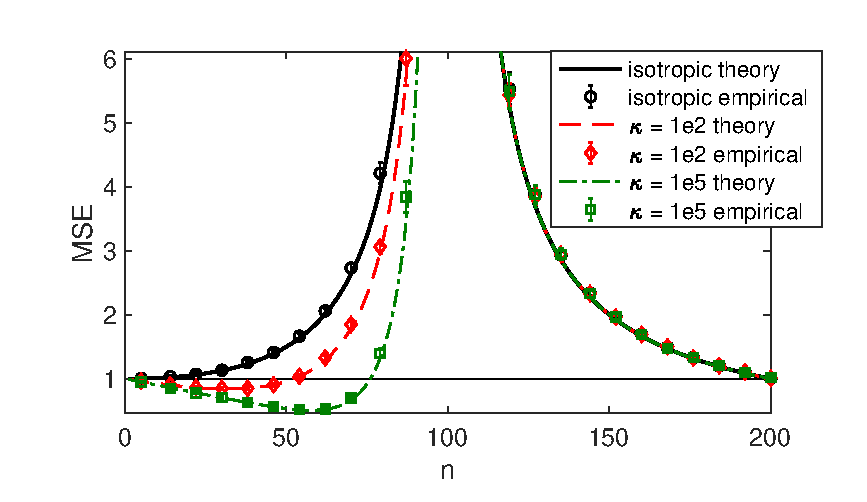
\includegraphics[width=0.48\textwidth]{figs/descent-intro}
  }
\hfill
\subfigure[%
    The mean of the estimator $\X^\dagger\y$ exhibits
    shrinkage which closely matches the shrinkage of a
    ridge-regularized least squares optimum (theory lines), as characterized by
    Theorem \ref{t:unbiased}.]{%
      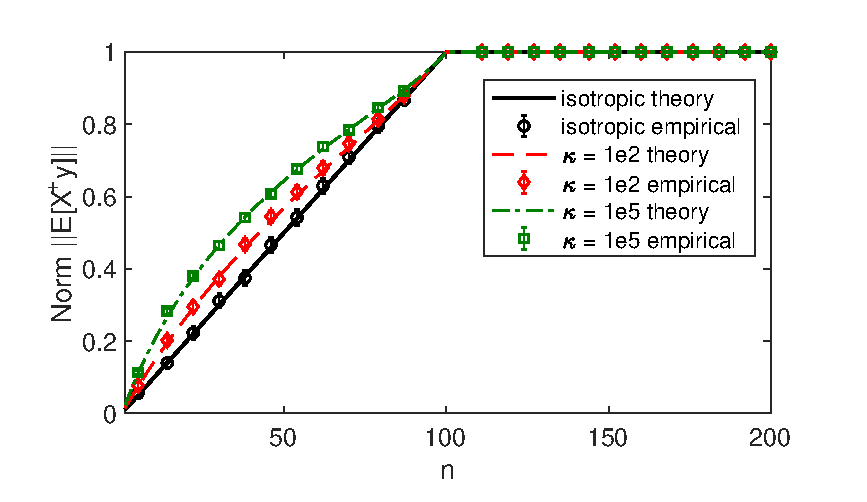
\includegraphics[width=0.48\textwidth]{figs/descent-shrinkage}
    }
\caption{Illustration of the main results for $d=100$ and
$\mu=\Nc(\zero,\Sigmab)$ where $\Sigmab$ is diagonal with
eigenvalues decaying exponentially and scaled so that
$\tr(\Sigmab^{-1})=d$. We use our surrogate
formulas to plot (a) the MSE (Theorem \ref{t:mse}) and (b) the norm of the expectation (Theorem
\ref{t:unbiased}) of the Moore-Penrose estimator (\emph{theory}
lines), accompanied by the empirical estimates based on the standard
i.i.d.~design (error bars are three times the standard error of the
mean). We consider three different condition numbers $\kappa$ of
$\Sigmab$, with \emph{isotropic} corresponding to $\kappa=1$,
i.e., $\Sigmab=\I$. We use $\sigma^2=1$ and
$\w^*=\frac1{\sqrt{d}}\one$.}
\vspace{-5mm}
\label{f:intro}
\end{figure}

\noindent
Proof of Theorem \ref{t:mse} is given in Appendix \ref{a:mse-proof}.
For illustration, we plot the MSE expressions in Figure~\ref{f:intro}a,
comparing them with empirical estimates of the true MSE under the
i.i.d.~design for a multivariate Gaussian distribution
$\mu=\Nc(\zero,\Sigmab)$ with several different covariance matrices $\Sigmab$. We keep the number of features $d$ fixed to
$100$ and vary the number of samples $n$, observing a double descent
peak at $n=d$. We observe that our theory aligns well with
the empirical estimates, whereas
previously, no such theory was available except for special
cases such as $\Sigmab=\I$ (more details in Theorem \ref{t:asymptotic}
and Appendices \ref{sec:proof-of-t-asymptotic} and \ref{sec:asymp-conj-details}). The plots
show that varying the spectral decay of $\Sigmab$ has a significant effect on the
shape of the curve in the under-determined regime. We use the
horizontal line to denote the MSE of the null estimator
$\mathrm{MSE}[\zero]=\|\w^*\|^2=1$. When the eigenvalues of $\Sigmab$
decay rapidly, then the Moore-Penrose estimator suffers less error
than the null estimator for some values of $n<d$, and the curve
exhibits a local optimum in this regime.

One important aspect of Theorem~\ref{t:mse} comes from the relationship between $n$ and the parameter $\lambda_n$, which together satisfy $n=\tr(\Sigmab_\mu (\Sigmab_\mu+\lambda_n\I)^{-1})$.
This expression is precisely the classical notion of \emph{effective
  dimension} for ridge regression regularized with
$\lambda_n$~\citep{ridge-leverage-scores}, and it arises here even though there is
no explicit ridge regularization in the problem being considered in
Theorem~\ref{t:mse}. 
The global solution to the ridge regression task (i.e., $\ell_2$-regularized
least squares) with parameter $\lambda$ is defined as:
\begin{align*}
\argmin_\w \Big\{\E_{\mu,y}\big[\big(\x^\top\w-y(\x)\big)^2\big]
    + \lambda\|\w\|^2\Big\}\ =\ (\Sigmab_\mu +
  \lambda\I)^{-1}\v_{\mu,y},\quad\text{where } \v_{\mu,y}=\E_{\mu,y}[y(\x)\,\x ].
\end{align*}
When Assumption \ref{a:linear} holds, then
$\v_{\mu,y}=\Sigmab_\mu\w^*$, however ridge-regularized least squares
is well-defined for much more general response models.
Our second result makes a direct connection between the (expectation
of the) unregularized minimum norm solution on the sample
and the global ridge-regularized solution.
While the under-determined regime (i.e., $n<d$) is of primary interest to us,
for completeness we state this result for arbitrary values of $n$ and $d$.
Note that, just like the definition of regularized least squares, this
theorem applies more generally than Theorem~\ref{t:mse}, in that it
does \emph{not} require the responses to follow any linear model as in
Assumption~\ref{a:linear} (proof in Appendix~\ref{s:unbiased-proof}). 
\begin{theorem}[Implicit regularization of Moore-Penrose estimator]
\label{t:unbiased}
For $\mu$ satisfying\footnote{The proof of Theorem \ref{t:unbiased}
  can be easily extended to probability measures $\mu$ that do not
  satisfy Assumption~\ref{a:general-position} (such as discrete distributions). We include this
  assumption here to simplify the presentation.} Assumption~\ref{a:general-position} and
  $y(\cdot)$ s.t.~$\v_{\mu,y}=\E_{\mu,y}[y(\x)\,\x]$ is well-defined, if
  $\Xb\sim S_\mu^n$ (Definition \ref{d:surrogate}) and $\yb_i=y(\xbb_i)$, then
  \begin{align*}
    \E\big[\Xb^\dagger\ybb\big] =
    \begin{cases}
       (\Sigmab_\mu + \lambda_n\I)^{-1}\v_{\mu,y} &\text{for }n<d,\\
        \Sigmab_\mu^{-1}\v_{\mu,y} &\text{for }n \ge d,
    \end{cases}
  \end{align*}
  where, as in Theorem \ref{t:mse}, $\lambda_n$ is such that the effective dimension
  $\tr(\Sigmab_\mu(\Sigmab_\mu+\lambda_n\I)^{-1})$ equals $n$.
\end{theorem}

\noindent
That is, when $n < d$, the Moore-Penrose estimator (which itself is
not regularized), computed on the
random training sample, in expectation equals the global ridge-regularized least
squares solution of the underlying regression
problem. Moreover, $\lambda_n$, i.e., the amount
of implicit $\ell_2$-regularization, is controlled by the degree of
over-parameterization in such a way as to ensure that $n$ becomes the ridge effective dimension
(a.k.a.~the effective degrees of freedom).

We illustrate this result in Figure
\ref{f:intro}b, plotting the norm of the expectation of the
Moore-Penrose estimator. As for the MSE, our surrogate theory aligns
well with the empirical estimates for i.i.d.~Gaussian designs, showing
that the shrinkage of the unregularized estimator in the
under-determined regime matches the implicit
ridge-regularization characterized by Theorem \ref{t:unbiased}. While the shrinkage
is a linear function of the sample size $n$ for isotropic features
(i.e., $\Sigmab=\I$), it
exhibits a non-linear behavior for other spectral decays.
Such \emph{implicit regularization} has been studied
previously~\citep[see, e.g.,][]{MO11-implementing, %PM11, GM14_ICML,
Mah12}; it has
been observed empirically for RandNLA sampling
algorithms~\citep{MMY15}; and it has also received attention more
generally within the context of neural networks~\citep{Ney17_TR}. While our implicit regularization result
is limited to the Moore-Penrose estimator, this new connection (and
others, described below) between the minimum norm solution of an unregularized
under-determined system and a ridge-regularized least squares solution
offers a simple interpretation for the implicit regularization
observed in modern machine learning architectures.

Our exact non-asymptotic expressions in Theorem~\ref{t:mse} and
our exact implicit regularization results in Theorem~\ref{t:unbiased}
are derived for the surrogate design, but Figure \ref{f:intro}
suggests that they accurately describe the MSE (up to lower order
terms) also under the standard i.i.d.~design $\X\sim\mu^n$,
particularly when $\mu$ is a multivariate Gaussian.
As a third result, we can verify this in the cases where there exist
known expressions for the MSE under the i.i.d.~design (standard
Gaussian for the under-determined setting, and
arbitrary Gaussian for the over-determined one).
We give the proof in Appendix~\ref{sec:proof-of-t-asymptotic}.
\begin{theorem}[Asymptotic consistency of surrogate design]
\label{t:asymptotic}
Let $\rho=n/d\neq 1$, $\X\sim \mu^n$
and $y_i=y(\x_i)$ satisfy Assumption~\ref{a:linear}. If $d\geq
c_\rho=\frac3{|1-\rho|}$ and
\begin{align*}
  \mu &= \begin{cases}
    \Nc(\zero,\I)&\text{when }n<d-1,\\
    \Nc(\zero,\Sigmab),\ \Sigmab\succ\zero &\text{when }n>d+1,
  \end{cases}
\end{align*}
then the absolute difference between surrogate
expressions and the true MSE is bounded as follows:
% &\text{if}\qquad  (1)\quad \rho<1\ \text{ and }\ \mu=\Nc(\zero,\I)\qquad\text{or}\qquad
%     (2)\quad \rho > 1\ \text{ and }\ \mu=\Nc(\zero,\Sigmab),\
%     \Sigmab\succ\zero,\\
\begin{align*}
\Big|\MSE{\X^\dagger\y}-\Mc(\Sigmab, \w^*,\sigma^2,n)\Big|\ \leq\
\frac{c_\rho}{d} \cdot \Mc(\Sigmab,\w^*,\sigma^2,n).
\end{align*}
\end{theorem}
\begin{remark}
For $n$ equal to $d-1$, $d$ or $d+1$, the true MSE under Gaussian
random design can be infinite, whereas the
surrogate MSE is finite and has a closed form expression.
\end{remark}

\noindent
Empirical estimates given in Figure
\ref{f:intro} suggest that the consistency of surrogate expressions
holds much more generally than it is stated above. Based on a detailed
empirical analysis described in Appendix \ref{sec:asymp-conj-details},
we conjecture that an asymptotic consistency 
result of the form similar to the statement of Theorem~\ref{t:asymptotic}
holds true in the under-determined regime without the assumption that
$\Sigmab=\I$ (see Conjectures \ref{c:wishart} and
\ref{c:projection}). In this case, no formula is known for 
$\MSE{\X^\dagger\y}$, whereas the expressions for the surrogate
Gaussian design naturally extend.

\subsection{Key techniques: surrogate designs and
  determinant preserving matrices}

The standard random design model for linear regression assumes that
each pair $(\x_i^\top,y_i)$ is drawn independently, where the row vector
$\x_i^\top$ comes from some $d$-variate distribution $\mu$ and $y_i=y(\x_i)$ is a random response variable drawn conditionaly on $\x_i$.
Precise theoretical analysis of under-determined regression in this
setting poses significant challenges, even in such special cases as
the Moore-Penrose estimator and a Gaussian data distribution $\mu$.
Rather than trying to directly analyze the usual i.i.d.~random design
$\X\sim\mu^n$ described above, we modify it slightly by introducing
the notion of a \emph{surrogate random design}, $\Xb\sim S_\mu^n$.
Informally, the goal of a surrogate random design is to modify an
original design to capture the main properties of the original design,
while being ``nicer'' for theoretical or empirical analysis.
In particular, here, we will modify the distribution of matrix $\X$ so
as to:
\begin{enumerate}
  \item closely preserve the behavior of the Moore-Penrose estimator
from the i.i.d.~design; and
  \item obtain exact expressions for double descent in terms of the
    mean squared error.
\end{enumerate}
A key element in the construction of our surrogate designs involves rescaling the measure $\X\sim\mu^n$ by the pseudo-determinant $\pdet(\X\X^\top)$, i.e., a product of the non-zero eigenvalues.
A similar type of determinantal design was suggested by
\cite{correcting-bias-journal}, but it was restricted there only to
$n\geq d$.
We broaden this definition by not only allowing the sample size to be
less than $d$, but also allowing it to be randomized.
A key property of our determinantal design matrix $\Xb$ is that
the expectation of a function $F(\Xb)$ can be, up to normalization,
expressed as:
\begin{align*}
  \E[F(\Xb)]\ \propto\ \E[\pdet(\X\X^\top)F(\X)],
  \end{align*}
where $\X\sim\mu^K$ and $K$ is a random variable (see details in Definition~\ref{d:det}).
Then, we define (in Definition~\ref{d:surrogate}) our surrogate design $S_\mu^n$ for each $n>0$ as a determinantal design with a carefully chosen random variable $K$, so that the expected sample size is equal to $n$ and so that it is possible to derive closed form expressions for the MSE.
We achieve this by using the Poisson distribution to construct the variable~$K$.

The key technical contribution that allows us to derive the MSE for determinantal designs is the concept of \emph{determinant preserving random matrices}, a notion that we expect to be useful more generally.
Specifically, in Section~\ref{s:dp} we define a class of $d\times d$ random
matrices $\A$ for which taking the determinant commutes with taking
the expectation, for the matrix itself and any of its square submatrices (see Definition~\ref{d:main}):
\begin{align*}
  \E\big[\!\det(\A_{\Ic,\Jc})\big] =
  \det\!\big(\E[\A_{\Ic,\Jc}]\big)\quad \text{for all }\Ic,\Jc\subseteq
  [d]\text{ s.t. }|\Ic|=|\Jc|.
\end{align*}
  Not all random matrices satisfy this property, however many
interesting and non-trivial examples can be found. Constructing
these examples is facilitated by the closure properties that this
class enjoys. In particular, if $\A$ and $\B$ are determinant
preserving and independent, then $\A+\B$ and $\A\B$ are also
determinant preserving (see Lemma \ref{t:ring}). We use these
techniques to prove a number of determinantal expectation
formulas needed in obtaining Theorems~\ref{t:mse}
and~\ref{t:unbiased}. For example, we show that if $\X\sim\mu^K$,
where $K$ is a Poisson random variable, then:
\begin{align*}
  \text{(Lemma \ref{l:poisson})}\quad  \E\big[\det(\X^\top\X)\big]
  &= \det\!\big(\E[\X^\top\X]\big),\\
\text{(Lemma \ref{l:normalization})}\quad  \E\big[\det(\X\X^\top)\big]
&= \ee^{-\E[K]}\det\!\big(\I + \E[\X^\top\X]\big).
\end{align*}

\section{Related work}
\label{s:related-work}

There is a large body of related work, which for simplicity we cluster into three groups.

\textbf{Double descent.}
The double descent phenomenon \cite[a term introduced by][]{BHMM19}
corresponds to the phase transition in the generalization error that
occurs when the ratio between the model complexity and the
sample size crosses the so-called interpolation threshold. It has been observed empirically
in a number of learning models, including neural networks
\citep{BHMM19,GJSx19_TR}, kernel methods \citep{BMM18_TR,BRT18_TR},
nearest neighbor models \citep{BHM18_TR}, and decision trees \citep{BHMM19}. The
theoretical analysis of double descent, and more broadly the generalization
properties of interpolating estimators, have primarily focused on various forms of
linear regression. The most comparable
to our work are \cite{BLLT19_TR,LR18_TR} and \cite{HMRT19_TR}, who provide
non-asymptotic upper/lower bounds and asymptotic formulas,
respectively, for the generalization error of the Moore-Penrose
estimator under essentially the same i.i.d.~random design setting as
ours. On the other hand, \cite{MVSS19_TR} provide bounds for the error
of the ideal linear interpolator (instead of the minimum norm
one). Note that while we analyze the classical mean squared error, many
works focus on the squared prediction error instead (some of them still
refer to it as the MSE).
Another line of literature deals with linear regression in the
so-called \emph{misspecified} setting, where the set of observed
features does not match the feature space in
which the response model is linear
\citep{belkin2019two,HMRT19_TR,Mit19_TR,MM19_TR}, e.g., when the
learner observes a random subset of $d$ features from a larger
population. This is an important distinction,
because it allows varying the model complexity by changing the number
of observed features while keeping the linear model fixed (see further
discussion in Section \ref{s:conclusions}). We believe
that our results can be extended to this important setting, and we leave
this as a direction for future work.

% Here are things to cite about double descent and related things.
% Original double descent papers:
% \cite{BHMM19}
% \cite{BMM18_TR}
% \cite{BRT18_TR}
% \cite{belkin2019two}
% Other double descent papers:
% \cite{AS17_TR}
% \cite{BLLT19_TR}
% \cite{BHM18_TR}
% \cite{BFF19_TR}
% \cite{COB18_TR}
% \cite{GJSx19_TR}
% \cite{HMRT19_TR}
% \cite{LR18_TR}
% \cite{MBB17_TR}
% \cite{MM19_TR}
% \cite{Mit19_TR}
% \cite{MVSS19_TR}
% \cite{NMBx18_TR}
% \cite{SKS18_TR}
% \cite{SGAx18_TR}
% \cite{WGSx19_TR}
% \michael{Say something about how we use MSE but others use one of a wide range of slightly different generalization metrics. Would you put in a draft, and then I can make a pass.}


\textbf{RandNLA.}
Randomized numerical linear algebra
\citep{DM16_CACM,RandNLA_PCMIchapter_TR} has
traditionally focused on obtaining algorithmic improvements for tasks
such as least squares and low-rank approximation via techniques that include
sketching \citep{sarlos-sketching} and i.i.d.~leverage score sampling
\citep{Drineas2006sampling}. However, there has been growing
interest in understanding the statistical properties of these
randomized methods \citep{MMY15,GarveshMahoney_JMLR}, for example
looking at the mean squared error of the least squares estimator
obtained via i.i.d.~subsampling under the standard linear response
model. Determinantal sampling methods (a.k.a.~volume sampling, or
determinantal point processes), which first found their way
into RandNLA in the context of low-rank approximation
\cite[][]{pca-volume-sampling}, have been recently shown to combine
strong worst-case guarantees with elegant statistical properties.
In particular, \cite{unbiased-estimates} showed that the
least-squares estimator subsampled via the so-called size $d$ volume
sampling (loosely corresponding to the special case of our surrogate design
$S_\mu^n$ where $n=d$) is an unbiased estimator that admits exact
formulas for both the expected square loss (a worst-case metric)
and the mean squared error (a statistical metric). These results were
developed further by
\cite{leveraged-volume-sampling,correcting-bias,minimax-experimental-design},
however they were still limited to the over-determined setting 
\cite[with the exception
of][who gave upper bounds on the mean squared error of the ridge estimator
under different determinantal
samplings]{regularized-volume-sampling,bayesian-experimental-design}.
Also in the over-determined setting, 
\cite{correcting-bias-journal} provided evidence for the fact that
determinantal rescaling can be used to modify the original data
distribution (particularly, a multivariate Gaussian) without a
significant distortion to the estimator, while making certain
statistical quantities expressible analytically. We take this
direction further by analyzing the unregularized least squares
estimator in the under-determined setting which is less well
understood, partly due to the presence of implicit regularization.

\textbf{Implicit regularization.}
The term implicit regularization typically refers to the notion that approximate
computation (e.g., rather than exactly minimizing a function $f$,
instead running an approximation algorithm to get an approximately
optimal solution) can implicitly lead to
statistical regularization (e.g., exactly minimizing an objective of
the form $f + \lambda g$, for some well-specified $\lambda$ and $g$).
See~\cite{MO11-implementing, PM11, GM14_ICML} and references therein
for early work on the topic; and see~\cite{Mah12} for an overview.
More recently, often motivated by neural networks, there has been work
on implicit regularization that typically considered SGD-based
optimization algorithms.
See, e.g., theoretical results on simplified
models~\citep{NTS14_TR,Ney17_TR,SHNx17_TR,GWBNx17,ACHL19,KBMM19_TR}
as well as extensive empirical and phenomenological results on state-of-the-art neural
network models~\citep{MM18_TR,MM19_HTSR_ICML}.
The implicit regularization observed by us is different in that it is
not caused by an inexact approximation algorithm (such as SGD) but rather by the
selection of one out of many exact solutions (e.g., the minimum norm
solution). In this context, most relevant are the
asymptotic results of~\cite{LJB19_TR} \cite[which used the asymptotic risk
results for ridge regression of][]{DW15_TR} and~\cite{KLS18_TR}.
Our non-asymptotic results are also related to recent work in
RandNLA on the expectation of the 
inverse~\citep{determinantal-averaging} and generalized
inverse~\citep{MDK19_TR} of a subsampled matrix.

\section{Surrogate random designs}
\label{s:determinantal}

In this section, we provide the definition of our surrogate random
design $S_\mu^n$, where $\mu$ is a $d$-variate probability measure and
$n$ is the sample size. This distribution is used in place
of the standard random design $\mu^n$ consisting of $n$ row vectors drawn
independently from $\mu$. Our surrogate design uses determinantal
rescaling to alter the joint distribution of the vectors so that
certain expected quantities (such as the mean squared error of the
Moore-Penrose estimator) can be expressed in a closed form.
We start by introducing notation.
%to be used throughout the rest of the paper.

%\paragraph{Preliminaries}
\textbf{Preliminaries.}
The set $\{1,...,n\}$ will be denoted by $[n]$.
For an $n\times n$ matrix $\A$, we use $\pdet(\A)$ to denote the pseudo-determinant of $\A$,
which is the product of non-zero eigenvalues. For index subsets $\Ic$
and $\Jc$, we use $\A_{\Ic,\Jc}$ to denote the submatrix of $\A$ with
rows indexed by $\Ic$ and columns indexed by $\Jc$. We may write
$\A_{\Ic,*}$ to indicate that we take a subset of rows. We use $\adj(\A)$ to
denote the adjugate of $\A$, defined as follows: the
$(i,j)$th entry of $\adj(\A)$ is
$(-1)^{i+j}\det(\A_{[n]\backslash\{j\},[n]\backslash\{i\}})$.
% We will
% use two useful identities related to the adjugate: (1)
% $\adj(\A)=\det(\A)\A^{-1}$ for invertible $\A$, and (2)
% $\det(\A+\u\v^\top)=\det(\A)+\v^\top\!\adj(\A)\u$.
% A formula called Sylvester's theorem
% relates the adjugate and the determinant: $\det(\A+\u\v^\top)=\det(\A)+\v^\top\!\adj(\A)\u$.
For a probability measure $\mu$ over $\R^d$, we use $\x^\top\!\sim\mu$
to denote a random row vector $\x^\top$ sampled according to this distibution.
We let $\X\sim\mu^k$ denote a $k\times d$ random matrix with rows
drawn i.i.d.~according to $\mu$, and the $i$th row is denoted as $\x_i^\top$.
We also let $\Sigmab_\mu=\E_{\mu}[\x\x^\top]$, where $\E_{\mu}$ refers to
the expectation with respect to $\x^\top\!\sim\mu$, assuming throughout that
$\Sigmab_\mu$ is well-defined and positive definite.
We use $\Poisson(\gamma)_{\leq a}$ as the Poisson distribution
restricted to $[0,a]$, whereas $\Poisson(\gamma)_{\geq a}$ is restricted
to $[a,\infty)$.
We also let $\#(\X)$ denote the number of rows of $\X$.

We now define a family of determinantal distributions over random matrices $\Xb$,
where not only the entries but also the number of rows is
randomized.
This randomized sample size is a crucial property of our
designs that enables our analysis.
% Our definition follows by
% expressing $\E[F(\Xb)]$ for real-valued functions $F:\bigcup_{k\geq 0}\R^{k\times
%   d}\rightarrow \R$ (the expectation may be undefined for some functions).
\begin{definition}\label{d:det}
  Let $\mu$ satisfy Assumption~\ref{a:general-position} and let $K$ be
  a random variable over non-negative integers. A determinantal design
    $\Xb\sim \Det(\mu,K)$ is a
distribution with the same domain as $\X\sim\mu^K$ such that~for any
event $E$ measurable w.r.t.~$\X$, we have
\begin{align*}
\Pr\big\{\Xb\in E\big\}\ = \frac{\E[\pdet(\X\X^\top)\one_{[\X\in E]}]}{\E[\pdet(\X\X^\top)]}.
\end{align*}
\end{definition}

\noindent
% Setting $F(\cdot)$ to 1, observe that the proportionality constant
% must be $1/\E[\pdet(\X\X^\top)]$.
The above definition can be
interpreted as rescaling the density function of $\mu^K$ by the
pseudo-determinant, and then renormalizing it.
We now construct our surrogate design $S_\mu^n$ by appropriately
selecting the random variable $K$.
The obvious choice of $K=n$ does \emph{not} result in simple closed form expressions for the MSE in the under-determined regime (i.e., $n<d$), which is the regime of primary interest to us.
Instead, we derive our random variables $K$ from the Poisson distribution.
\begin{definition}\label{d:surrogate}
For $\mu$ satisfying Assumption~\ref{a:general-position},
define surrogate design $S_\mu^n$ as $\Det(\mu,K)$ where:
\vspace{-2mm}
    \begin{enumerate}
\item if $n<d$, then $K\sim \Poisson(\gamma_n)_{\leq d}$ with
 $\gamma_n$ being the solution of
 $n=\tr(\Sigmab_\mu(\Sigmab_\mu+\frac1{\gamma_n}\I)^{-1})$,
 \vspace{-2mm}
\item if $n=d$, then we simply let $K=d$,
  \vspace{-2mm}
\item if $n>d$, then $K\sim\Poisson(\gamma_n)_{\geq d}$ with $\gamma_n=n-d$.
\end{enumerate}
\end{definition}

\noindent
Note that the under-determined case, i.e., $n<d$, is restricted to $K\leq d$ so that, under Assumption~\ref{a:general-position}, $\pdet(\X\X^\top)=\det(\X\X^\top)$ with probability 1.
On the other hand in the over-determined case, i.e., $n>d$, we have
$K\geq d$ so that $\pdet(\X\X^\top)=\det(\X^\top\X)$. In the special case
of $n=d=K$ both of these equations are satisfied: $\pdet(\X\X^\top)=\det(\X^\top\X)=\det(\X\X^\top)=\det(\X)^2$.

The first non-trivial property of the surrogate design $S_\mu^n$ is
that the expected sample size is in fact always equal to $n$, which we
prove in Appendix \ref{appx: proof-of-l-size}.
\begin{lemma} \label{l:size}
Let $\Xb\sim S_\mu^n$ for any $n>0$.
 Then, we have $\E[\#(\Xb)] = n$.
\end{lemma}

\noindent
 Our general template for computing expectations under
 a surrogate design $\Xb\sim\S_\mu^n$ is to use the following expressions based on the
i.i.d.~random design $\X\sim\mu^K$:
\begin{align}
  \E[F(\Xb)] &=\begin{cases}
    \frac{\E[\det(\X\X^\top)F(\X)]}{\E[\det(\X\X^\top)]}
   \quad K\sim\Poisson(\gamma_n)&\text{for }n<d,\\[2mm]
    \frac{\E[\det(\X)^2F(\X)]}{\E[\det(\X)^2]}\hspace{3mm}
    \quad K=d&\text{for }n=d,\\[2mm]
    \frac{\E[\det(\X^\top\X)F(\X)]}{\E[\det(\X^\top\X)]}
   \quad K\sim\Poisson(\gamma_n)&\text{for }n>d.
  \end{cases}\label{eq:cases}
\end{align}
These formulas follow from Definitions \ref{d:det} and
\ref{d:surrogate} because the determinants $\det(\X\X^\top)$ and
$\det(\X^\top\X)$ are non-zero precisely in the regimes $n\leq d$ and
$n\geq d$, respectively, which is why we can drop the restrictions on the
range of the Poisson distribution.
The normalization constants for computing the expectations
can be obtained using the following formulas: if $\X\sim\mu^K$ then
\begin{align*}
\text{(Lemma~\ref{l:normalization})}&&
\E\big[\det(\X\X^\top)\big]  &= \ee^{-\gamma_n}\det(\I +
\gamma_n\Sigmab_\mu)&&\text{for } K\sim\Poisson(\gamma_n),\ n<d,\\
  \text{(Lemma~\ref{l:cb})}&& \E\big[\det(\X)^2\big] &=
  d!\det(\Sigmab_\mu),&&\text{for } K=n=d,\\
  \text{(Lemma~\ref{l:poisson})}&& \E\big[\det(\X^\top\X)\big]
&=\det(\gamma_n\Sigmab_\mu),&&  \text{for }K\sim\Poisson(\gamma_n),\ n>d.
\end{align*}
% \begin{remark}
% We will use $Z_\mu^n$ as a shorthand for the above normalization constants.
% \end{remark}
% For the case of $n=d$, the normalization constant can be found in the
% literature \cite{expected-generalized-variance,correcting-bias}:
We prove Lemmas \ref{l:poisson} and \ref{l:normalization} in Section
\ref{s:dp} by introducing the
concept of determinant preserving random matrices.
% The lemmas play a
% crucial role in deriving a number of new expectation formulas for the
% under- and over-determined surrogate designs that we use to prove Theorems~\ref{t:mse}
% and~\ref{t:unbiased} in Section~\ref{s:expectations}.
On the other hand, Lemma  \ref{l:cb} and the design $S_\mu^d$ can be found in the
literature \citep{expected-generalized-variance,correcting-bias-journal},
and we will rely on those known results in this case.
% Importantly, the $n=d$ case offers a continuous transition between the under-
% and over-determined regimes because the distribution $S_\mu^n$
% converges to $S_\mu^d$ when $n$ approaches $d$ from above and
% below.

We now highlight some key expectation formulas for surrogate designs, which are used to
derive the MSE expressions from Theorem \ref{t:mse}. A standard decomposition of
the MSE yields:% for the Moore-Penrose estimator yields:
\begin{align}
  \MSE{\Xb^\dagger\ybb}
  &= \E\big[\|\Xb^\dagger(\Xb\w^*+\xib)-\w^*\|^2\big]
  =\sigma^2\E\big[\tr\big((\Xb^\top\Xb)^{\dagger}\big)\big] +
    \w^{*\top}\E\big[\I-\Xb^\dagger\Xb\big]\w^*.\label{eq:mse-derivation}
\end{align}
Thus, our task is to find closed form expressions for the two
expectations above. If $n\geq d$, then the latter goes away because
$\Xb^\dagger\Xb$ is the projection onto the row-span of $\Xb$ so
when $\Xb$ has rank $d$ then $\I-\Xb^\dagger\Xb=\zero$. When
$n<d$, it is given in the following result (proof in
Appendix \ref{s:unbiased-proof}).
% can be obtained as a consequence of Lemma \ref{l:ridge-under}.
\begin{lemma}\label{l:proj}
If  $\Xb\sim S_\mu^n$ and $n<d$, then we have:
$\E\big[\I-\Xb^\dagger\Xb\big] = (\gamma_n\Sigmab_\mu+\I)^{-1}$.
\end{lemma}

\noindent
No such expectation formula is known for i.i.d.~designs, except when
$\mu$ is an isotropic Gaussian. In Appendix \ref{s:unbiased-proof}, we
also prove a generalization of Lemma \ref{l:proj} which is then used
to establish our implicit regularization result
(Theorem~\ref{t:unbiased}). We next give an expectation formula 
for the trace of the Moore-Penrose inverse of the covariance
matrix for a surrogate design (proof in Appendix \ref{a:mse-proof}).
\begin{lemma}\label{l:sqinv-all}
If  $\Xb\sim S_\mu^n$, then:\vspace{-2mm}
\begin{align*}
    \E\big[\tr\big((\Xb^\top\Xb)^{\dagger}\big)\big]
  &=
    \begin{cases}
\gamma_n\big(1-
\det\!\big((\tfrac1{\gamma_n}\I+\Sigmab_\mu)^{-1}\Sigmab_\mu\big)\big),
&\text{for }n<d,\\
\tr(\Sigmab_\mu^{-1}),
&\text{for }n=d,\\
\tr(\Sigmab_\mu^{-1})\,\frac{1-\ee^{-\gamma_n}}{\gamma_n},
&\text{for }n>d.
\end{cases}
\end{align*}
\end{lemma}

\noindent
% The case of $n=d$ in the above lemma was shown by
% \cite{correcting-bias-journal} in Theorem~2.12, whereas the case of $n>d$
% is closely related to their Theorem 2.9.
Our key contribution is the under-determined
regime (i.e., $n<d$), where we observe implicit regularization
given by $\lambda_n=\frac1{\gamma_n}$. Since $n =
\tr(\Sigmab_\mu(\Sigmab_\mu+\lambda_n\I)^{-1})=d-\lambda_n\tr((\Sigmab_\mu+\lambda_n\I)^{-1})$,
it follows that $\lambda_n=(d-n)/\tr((\Sigmab_\mu+\lambda_n\I)^{-1})$.
Combining this with Lemmas \ref{l:proj} and \ref{l:sqinv-all}, we
recover the surrogate MSE expression in Theorem~\ref{t:mse} (see details
in Appendix \ref{a:mse-proof}).


\section{Determinant preserving random matrices}
\label{s:dp}

In this section, we introduce the key tool for computing expectation formulas of matrix determinants.
It is used in our analysis of the surrogate design, and it should be of independent interest.

The key question motivating the following definition is: When does taking expectation commute with computing a determinant for a square random matrix?
\begin{definition}\label{d:main}
A random $d\times d$ matrix $\A$ is called determinant
  preserving (d.p.), if
\begin{align*}
  \E\big[\!\det(\A_{\Ic,\Jc})\big] =
  \det\!\big(\E[\A_{\Ic,\Jc}]\big)\quad \text{for all }\Ic,\Jc\subseteq
  [d]\text{ s.t. }|\Ic|=|\Jc|.
\end{align*}
\end{definition}

\noindent
Note that from the definition of an adjugate matrix (see preliminaries
in Section \ref{s:determinantal}) it immediately follows that if $\A$ is
determinant preserving then adjugate commutes with expectation for this matrix:
\begin{align}
  \E\big[\big(\!\adj(\A)\big)_{i,j}\big] &=
  \E\big[(-1)^{i+j}\det(\A_{[d]\backslash\{j\},[d]\backslash\{i\}})\big]\nonumber
  \\
&=(-1)^{i+j}\det\!\big(\E[\A_{[d]\backslash\{j\},[d]\backslash\{i\}}]\big)
  = \big(\!\adj(\E[\A])\big)_{i,j}.\label{eq:adj}
\end{align}
The adjugate is useful in our analysis because it connects the
determinant and the inverse via the formula
$\adj(\A)=\det(\A)\A^{-1}$, which holds for any invertible $\A$.
We next give a few simple examples to provide some intuition. First, note
that every $1\times 1$ random matrix is determinant preserving simply
because taking a determinant is an identity transfomation in one
dimension. Similarly, every fixed matrix is determinant preserving because
in this case taking the expectation is an identity
transformation. In all other cases, however, Definition \ref{d:main}
has to be verified more carefully. Further examples (positive and
negative) follow.
\begin{example}
If $\A$ has i.i.d. Gaussian entries $a_{ij}\sim\Nc(0,1)$, then
$\A$ is d.p.~because $\E[\det(\A)]=0$.
\end{example}

\noindent
In fact, it can be shown that all random matrices with independent entries
are determinant preserving. However, this is not a necessary condition.
\begin{example}\label{e:rank-1}
Let $\A = s\,\Z$, where $\Z$ is fixed with $\rank(\Z) = r$, and $s$
is a scalar random variable. Then for $|\Ic|=|\Jc|=r$ we have
\begin{align*}
  \E\big[\det(s\,\Z_{\Ic,\Jc})\big] &= \E[s^r]\det(\Z_{\Ic,\Jc})
                                      =\det\Big(\big(\E[s^r]\big)^{\frac1r}\,\Z_{\Ic,\Jc}\Big),
\end{align*}
  so if $r=1$ then $\A$ is determinant preserving, whereas if $r>1$
  and $\Var[s]>0$ then it is not.
\end{example}

\noindent
To construct more complex examples, we show that determinant preserving random matrices are
closed under addition and multiplication. The proof of this result is
an extension of an existing argument, given by
\cite{determinantal-averaging} in the proof of Lemma~7, for computing
the expected determinant of the sum of rank-1 random matrices (proof in Appendix \ref{a:dp}). 
\begin{lemma}[Closure properties]\label{t:ring}
  If $\A$ and $\B$ are independent and determinant preserving, then:
  \begin{enumerate}
  \item $\A+\B$ is determinant preserving,
  \item $\A\B$ is determinant preserving.
    \end{enumerate}
\end{lemma}
% \begin{lemma}\label{t:ring}
%   If $\A,\B$ are independent and d.p.~then
%   $\A+\B$ and $\A\B$ are also determinant preserving.
% \end{lemma}

\noindent
Next, we introduce another important class of d.p.~matrices:
a sum of i.i.d.~rank-1 random matrices with the number of
i.i.d.~samples being a Poisson random variable. Our use of the Poisson
distribution is crucial for the below result to hold. It is an
extension of an expectation formula given by \cite{dpp-intermediate}
for sampling from discrete distributions (proof in Appendix \ref{a:dp}).
\begin{lemma}\label{l:poisson}
If $K$ is a Poisson random variable and $\A,\B$ are random $K\times d$
matrices whose rows  are sampled as an i.i.d.~sequence of joint pairs of
random vectors, then $\A^\top\B$ is d.p., and so:
\begin{align*}
  \E\big[\det(\A^\top\B)\big] &= \det\!\big(\E[\A^\top\B]\big).
  \end{align*}
\end{lemma}

\noindent
Finally, we show the expectation formula needed for obtaining the
normalization constant of the under-determined surrogate design, given
in \eqref{eq:cases}.
The below result is more general than the normalization constant
requires, because it allows the matrices $\A$ and $\B$ to be different
(the constant is obtained by setting $\A=\B=\X\sim\mu^K$).
In fact, we use this more general statement to show Theorems
\ref{t:mse} and~\ref{t:unbiased}. The proof uses
Lemmas \ref{t:ring} and \ref{l:poisson} (see Appendix \ref{a:dp}).
\begin{lemma}\label{l:normalization}
If $K$ is a Poisson random variable and $\A$, $\B$ are random $K\times d$
matrices whose rows  are sampled as an i.i.d.~sequence of joint pairs of
random vectors, then
\begin{align*}
  \E\big[\det(\A\B^\top)\big] &= \ee^{-\E[K]}\det\!\big(\I + \E[\B^\top\A]\big).
  \end{align*}
\end{lemma}


\section{Conclusions and open problems}
\label{s:conclusions}

We derived exact non-asymptotic expressions for the MSE of the
Moore-Penrose estimator in the standard regression task, reproducing
the double descent phenomenon as the sample size crosses between the
under- and over-determined regime. To achieve this, we modified the
standard i.i.d.~random design distribution using a determinantal
rescaling to obtain a surrogate design which admits exact MSE expressions,
while capturing the key properties of the i.i.d.~design. We
also provided a result that relates the expected value of the
Moore-Penrose estimator of a training sample in the under-determined regime (i.e., the
minimum norm solution) to the ridge-regularized least squares solution
for the population distribution, thereby providing an interpretation for the
implicit regularization resulting from over-parameterization.

\begin{wrapfigure}{r}{\ifisarxiv 0.5\else 0.47\fi\textwidth}
 \ifisarxiv\else \vspace{-.3cm}\fi
  \centering
 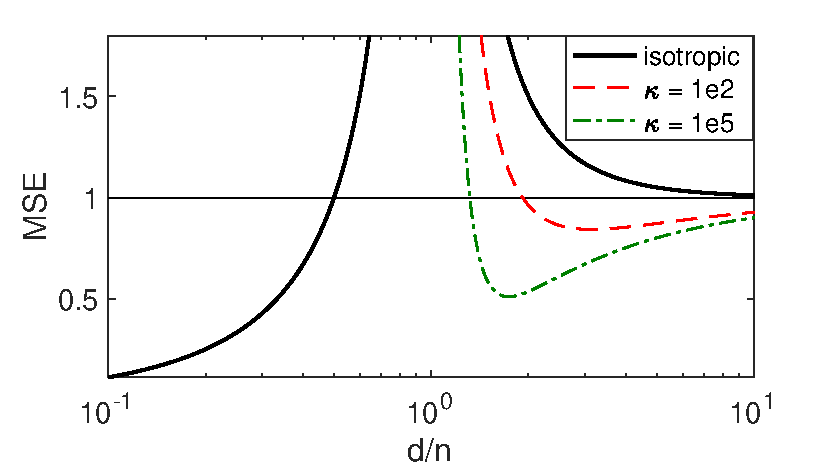
\includegraphics[width=.46\textwidth]{figs/descent-model-log}
\ifisarxiv\else \vspace{-2mm}\fi
  \caption{
Surrogate MSE as a function of $d/n$, with $n$
fixed to $100$ and varying $d$.}
  \label{f:model}
\ifisarxiv\else  \vspace{-.5cm}\fi
\end{wrapfigure}

An important technical issue is that, in this work, we focus on the classical \emph{well-specified}
linear regression task, where the underlying response model is linear
with respect to the observed feature space. A significant effort in
the related literature (see Section \ref{s:related-work}) has been
directed towards a number of \emph{misspecified} linear regression
tasks, where the set of $d$ observed features is different than the
set of $D$ features which define the linear model (typically, $d\ll
D$). Crucially, unlike in the well-specified task, here it is possible
to vary the number of observed features without changing the
underlying linear model.
Recent work \citep{HMRT19_TR} has compared how
varying the feature dimension affects the (asymptotic) generalization
error for both well-specified and misspecified tasks, however their
analysis was limited to certain special settings such as an
isotropic data distribution. As an additional
point of comparison, in Figure~\ref{f:model} we plot the MSE
expressions of Theorem~\ref{t:mse} for our well-specified setting when varying the
feature dimension~$d$. The model is chosen just like in
Figure~\ref{f:intro}, where the covariances $\Sigmab_\mu$ are diagonal
with condition number $\kappa$ and exponentially decaying spectrum
scaled so that $\tr(\Sigmab_\mu^{-1})=d$. We also use $\sigma^2=1$ and
$\w^*=\frac1{\sqrt{d}}\one$. Qualitatively, our plots follow the
trends outlined by \cite{HMRT19_TR} for the isotropic case (i.e., $\kappa=1$),
but the spectral decay of the covariance matrix (captured by our new
MSE expressions) does have a significant effect on the descent curve
in the under-determined regime. Note that the plots achieve their
minimum as $d$ goes to zero because in the well-specified task as
the complexity of the prediction model decreases, so does the complexity of the
true response model. Nevertheless,
we observe generalization in the under-determined regime,
as seen by the fact that the MSE curve goes below the error of the
null estimator, $\mathrm{MSE}[\zero]=1$.


Our work opens up a number of new directions for future research.
This includes extending our surrogate analysis to the
misspecified linear regression discussed above.
Also, it remains open whether the analysis we provided for the mean
squared error can be reproduced in the context of mean squared
\emph{prediction} error, which is relevant in many machine learning
tasks. Finally, while Theorem \ref{t:asymptotic} states that our surrogate
expressions for the MSE under certain Gaussian designs are
asymptotically consistent with the multiplicative error rate of
$O(1/d)$, we believe that this fact extends to
the setting not covered by the theorem: under-determined regime (i.e.,
$n<d$) with a non-isotropic Gaussian distribution (i.e., $\Sigmab\neq
\I$). We break down our analysis into verifying two
conjectures which are of independent interest to multivariate
Gaussian analysis. The first conjecture addresses the first term in
the MSE derivation \eqref{eq:mse-derivation} and postulates an asymptotically
consistent formula for the expected Moore-Penrose inverse
of the pseudo-Wishart distribution. Matrix
$\W\sim\Pc\Wc(\Sigmab,n)$ is distributed according to the pseudo-Wishart
distribution with $n<d$ degrees of freedom \citep{srivastava1979introduction} if it can be written as
$\W=\X^\top\X$, where $\X\sim\Nc_{n,d}(\zero, \I_n \otimes \Sigmab)$
is the matrix-variate Normal \citep{gupta2018matrix}, i.e., an
i.i.d.~Gaussian design.
% we call it a pseudo-Wishart 
% and write $\W \sim \Pc\Wc(\Sigmab, n)$
% if $n<d$ but still
\ifisarxiv\pagebreak\fi
\begin{conjecture}[Moore-Penrose inverse of pseudo-Wishart]\label{c:wishart}
  Fix $n/d<1$ and let $\W\sim\Pc\Wc(\Sigmab,n )$, where
$\Sigmab$ is $d\times d$ positive definite with condition number bounded by a constant.
Then:
\begin{align}
\bigg|\frac{\E\big[\tr(\W^\dagger)\big]}{\Vc(\Sigmab,n)} -1\bigg|=
  O(1/d)\qquad\text{for}\quad\Vc(\Sigmab,n)=\frac{1-\alpha_n}{\lambda_n},\label{eq:wishart}
\end{align}
where $\lambda_n\geq 0$ satisfies $n=\tr(\Sigmab(\Sigmab+\lambda_n\I)^{-1})$ and
$\alpha_n=\det(\Sigmab(\Sigmab+\lambda_n\I)^{-1})$.
\end{conjecture}

\noindent
Our second conjecture involves the projection onto the
orthogonal complement of a Gaussian sample $\X$, i.e., the matrix
$\I-\X^\dagger\X$, and addresses
the second term in the MSE derivation \eqref{eq:mse-derivation}.
\begin{conjecture}[Gaussian orthogonal projection]\label{c:projection}
  Fix $n/d<1$ and let $\X\sim \Nc_{n,d}(\zero,\I_n \otimes \Sigmab)$, where
$\Sigmab$ is $d\times d$ positive definite with condition number
bounded by a constant. Then:
\begin{align}
\sup_{\w\in\R^d\backslash\{\zero\}}\bigg|\frac{\w^\top\E[\I-\X^\dagger\X]\w}{\w^\top
  \Bc(\Sigmab,n)\w} - 1\bigg| = O(1/d)\qquad\text{for}\quad
  \Bc(\Sigmab,n) =
  \lambda_n(\Sigmab+\lambda_n\I)^{-1}.\label{eq:projection}
\end{align}
\end{conjecture}
% Note that the surrogate expression for the mean squared
% error can be written as:
% \[
% \Mc(\Sigmab_\mu,\w^*,\sigma^2,n)=\sigma^2 \Vc(\Sigmab_\mu,n)
% + \w^{*\top}\Bc(\Sigmab_\mu,n)\w^*.
% \]
% So, if the conjectures are true,
% this would immediately imply that the asymptotic consistency claim
% given in Theorem \ref{t:asymptotic} for
% the surrogate Gaussian MSE extends to
% the under-determined setting with arbitrary covariance $\Sigmab$.

\noindent
Recall that $\lambda_n=\frac {d-n}{\tr((\Sigmab+\lambda_n\I)^{-1})}$,
so our surrogate MSE is recovered as
$\sigma^2\Vc(\Sigmab,n)+\w^{*\top}\Bc(\Sigmab,n)\w^*$. 
% The expressions $\Vc(\Sigmab,n)$ and $\Bc(\Sigmab,n)$ and recover
% surrogate MSE from Theorem \ref{t:mse} since $\lambda_n=\frac{\tr((\Sigmab+\lambda_n)^{-1})}{d-n}$.
Conjectures \ref{c:wishart} and \ref{c:projection} provide new insights into classical matrix-variate
distributions with extensive literature dedicated to them \citep[see,
e.g.,][]{chikuse1990matrix,cook2011}. We discuss 
this further in Appendix \ref{sec:asymp-conj-details},
where we also provide detailed empirical evidence supporting these claims.

% In Appendix \ref{sec:asymp-conj-details} we provide further discussion
% and detailed empirical evidence for these conejctures.
% We believe that addressing these conjecture will have a broader
% impact on our understanding of non-isotropic Gaussian designs. 




% In addition, in Section \ref{s:asymptotic}, we provided two conjectures, the goal of which is to bound the difference between the results obtained for our surrogate designs and the true values corresponding to the i.i.d.~design, in the case of multivariate Gaussians.


\paragraph{Acknowledgements.}
We would like to acknowledge ARO, DARPA, NSF, ONR, and GFSD for providing
partial support of this work.

\ifisarxiv\bibliographystyle{plainnat}\fi
\bibliography{../pap}

\appendix




\section{Proof of Lemma~\ref{l:size}}
\label{appx: proof-of-l-size}

We first record an important property of the design $S_\mu^d$
which can be used to construct an over-determined design for any $n>d$. A similar
version of this result was also previously shown by
\cite{correcting-bias-journal} for a different determinantal design.

\begin{lemma}\label{l:decomposition}
  Let $\Xb\sim S_\mu^d$ and $\X\sim \mu^K$, where
  $K\sim\Poisson(\gamma)$. Then the matrix composed of a random
  permutation of the rows from $\Xb$ and $\X$ is distributed according to
  $S_\mu^{d+\gamma}$.
\end{lemma}

\begin{proof}
Let $\Xt$ denote the matrix constructed from the permuted rows of
$\Xb$ and $\X$.  Letting $\Z\sim\mu^{K+d}$, we derive the probability
$\Pr\big\{\Xt\!\in\! E\big\}$ by summing over the possible index subsets  $S\subseteq
[K+d]$ that correspond to the rows coming from $\Xb$:
\begin{align*}
  \Pr\big\{\Xt\in E\big\} &= \E\bigg[\frac{1}{\binom{K+d}{d}}
  \sum_{S:\,|S|=d}\frac{\E[\det(\Z_{S,*})^2\one_{[\Z\in E]}\mid
  K]}{d!\det(\Sigmab_\mu)}\bigg]\\
  &=\sum_{k=0}^\infty
    \frac{\gamma^k\ee^{-\gamma}}{k!}\,\frac{\gamma^dk!}{(k+d)!}\,
    \frac{\E\big[\sum_{S:\,|S|=d}\det(\Z_{S,*})^2\one_{[\Z\in E]}\mid
    K=k\big]}{\det(\gamma\Sigmab_\mu)}\\
  &\overset{(*)}{=} \sum_{k=0}^\infty
    \frac{\gamma^{k+d}\ee^{-\gamma}}{(k+d)!}
    \,\frac{\E[\det(\Z^\top\Z)\one_{[\Z\in E]}\mid K=k]}{\det(\gamma\Sigmab_\mu)},
\end{align*}
where $(*)$ uses the Cauchy-Binet formula to sum over all subsets $S$
of size $d$. Finally, since the sum shifts from $k$
to $k+d$, the last expression can be rewritten as
$\E[\det(\X^\top\X)\one_{[\X\in E]}]/\det(\gamma\Sigmab_\mu)$, where recall that
$\X\sim\mu^K$ and $K\sim\Poisson(\gamma)$, matching the definition of $S_\mu^{d+\gamma}$.
\end{proof}

We now proceed with the proof of Lemma \ref{l:size}, where we establish
that the expected sample size of $S_\mu^n$ is indeed $n$.

\begin{proofof}{Lemma}{\ref{l:size}}
  The result is obvious when $n=d$, whereas
  for $n>d$ it is an immediate consequence
  of Lemma \ref{l:decomposition}.
  Finally, for $n<d$ the expected sample
  size follows as a corollary of Lemma \ref{l:proj}, which states that
  \begin{align*}
\text{(Lemma \ref{l:proj})} \qquad\E\big[\I - \Xb^\dagger\Xb\big] =
    (\gamma_n\Sigmab_\mu + \I)^{-1},
  \end{align*}
  where $\Xb^\dagger\Xb$ is the orthogonal projection onto
  the subspace spanned by the rows of $\Xb$. Since the rank of this
  subspace is equal to the number of the rows, we have
  $\#(\Xb)=\tr(\Xb^\dagger\Xb)$, so
  \begin{align*}
    \E\big[\#(\Xb)\big] = d - \tr\big((\gamma_n\Sigmab_\mu +
    \I)^{-1}\big) =
    \tr\big(\gamma_n\Sigmab_\mu(\gamma_n\Sigmab_\mu+\I)^{-1}\big) = n,
  \end{align*}
  which completes the proof.
\end{proofof}

\section{Proofs for Section \ref{s:dp}}
\label{a:dp}

We use $\adj(\A)$ to denote the adjugate of $\A$, defined as follows: the
$(i,j)$th entry of $\adj(\A)$ is
$(-1)^{i+j}\det(\A_{[n]\backslash\{j\},[n]\backslash\{i\}})$.
We will use two useful identities related to the adjugate: (1)
$\adj(\A)=\det(\A)\A^{-1}$ for invertible $\A$, and (2)
$\det(\A+\u\v^\top)=\det(\A)+\v^\top\!\adj(\A)\u$
\citep[see Fact 2.14.2 in][]{matrix-mathematics}.

First, note that from the definition of an adjugate matrix it immediately follows that if $\A$ is
determinant preserving then adjugate commutes with expectation for this matrix:
\begin{align}
  \E\big[\big(\!\adj(\A)\big)_{i,j}\big] &=
  \E\big[(-1)^{i+j}\det(\A_{[d]\backslash\{j\},[d]\backslash\{i\}})\big]\nonumber
  \\
&=(-1)^{i+j}\det\!\big(\E[\A_{[d]\backslash\{j\},[d]\backslash\{i\}}]\big)
  \\
  &= \big(\!\adj(\E[\A])\big)_{i,j}.\label{eq:adj}
\end{align}
% The adjugate is useful in our analysis because it connects the
% determinant and the inverse via the formula
% $\adj(\A)=\det(\A)\A^{-1}$, which holds for any invertible $\A$.


\begin{proofof}{Lemma}{\ref{t:ring}} \
 First, we show that $\A+\u\v^\top$ is d.p.~for any fixed
 $\u,\v\in\R^d$. Below, we use the identity for a rank one
 update of a determinant:
 $\det(\A+\u\v^\top)=\det(\A)+\v^\top\!\adj(\A)\u$. It follows that
 for any $\Ic$ and $\Jc$ of the same size,
  \begin{align*}
\E\big[\!\det(\A_{\Ic,\Jc}\!+\u_{\Ic}\v_{\Jc}^\top)\big] &=
    \E\big[\!\det(\A_{\Ic,\Jc}) +
    \v_{\Jc}^\top\adj(\A_{\Ic,\Jc}) \u_{\Ic}\big]\\
    &\overset{(*)}{=}\det\!\big(\E[\A_{\Ic,\Jc}]\big) +
      \v_{\Jc}^\top\adj\!\big(\E[\A_{\Ic,\Jc}]\big) \u_{\Ic}\\
    &=\det\!\big(\E[\A_{\Ic,\Jc} \!+ \u_{\Ic}\v_{\Jc}^\top]\big),
  \end{align*}
  where $(*)$ used \eqref{eq:adj}, i.e., the fact that for d.p.~matrices, adjugate commutes
  with expectation. Crucially, through the definition of an adjugate
  this step implicitly relies on the assumption that all the square
  submatrices of $\A_{\Ic,\Jc}$ are also  determinant preserving.
  Iterating this, we get that $\A+\Z$ is d.p.~for any fixed
  $\Z$. We now show the same for $\A+\B$:
  \begin{align*}
\E\big[\!\det(\A_{\Ic,\Jc}\!+\B_{\Ic,\Jc})\big]
    &=
      \E\Big[\E\big[\!\det(\A_{\Ic,\Jc}\!+\B_{\Ic,\Jc})\mid\B\big]\Big]\\
    &\overset{(*)}{=}\E\Big[\!\det\!\big(\E[\A_{\Ic,\Jc}]\!+\B_{\Ic,\Jc}\big)\Big]\\
      &= \det\!\big(\E[\A_{\Ic,\Jc}\!+\B_{\Ic,\Jc}]\big),
  \end{align*}
  where $(*)$  uses the fact that after conditioning on $\B$ we can
  treat it as a fixed matrix. Next, we show that $\A\B$ is determinant preserving via the Cauchy-Binet formula:
  \begin{align*}
    \E\big[\!\det\!\big((\A\B)_{\Ic,\Jc}\big)\big]
    &= \E\big[\!\det(\A_{\Ic,*}\B_{*,\Jc})\big]\\
    &=\E\bigg[\sum_{S:\,|S|=|\Ic|}\!\!\det\!\big(\A_{\Ic,S}\big)
      \det\!\big(\B_{S,\Jc}\big)\bigg]\\
&=\!\!\sum_{S:\,|S|=|\Ic|}\!\!\det\!\big(\E[\A]_{\Ic,S}\big)
                                                \det\!\big(\E[\B]_{S,\Jc}\big)\\
    &=\det\!\big(\E[\A]_{\Ic,*}\, \E[\B]_{*,\Jc}\big)\\
      &= \det\!\big(\E[\A\B]_{\Ic,\Jc}\big),
  \end{align*}
  where recall that $\A_{\Ic,*}$ denotes the submatrix of $\A$
  consisting of its (entire) rows indexed by $\Ic$.
  \end{proofof}

To prove Lemma \ref{l:poisson}, we will use the following
lemma, many variants of which appeared in the literature
\cite[e.g.,][]{expected-generalized-variance}. We use the one given by
\cite{correcting-bias}.
\begin{lemma}[\cite{correcting-bias}]\label{l:cb}
If the rows of random $k\times d$ matrices $\A,\B$
  are sampled as an i.i.d.~sequence of $k\geq d$ pairs of joint random vectors, then
\begin{align}
  k^d\,\E \big[\det(\A^\top\B)\big]
  &= \ktd\,\det\!\big(\E[\A^\top\B]\big).
     \end{align}
 \end{lemma}

\noindent
Here, we use the following standard shorthand: $\ktd =
\frac{k!}{(k-d)!} = k\,(k-1)\dotsm(k-d+1)$. Note that the above result
almost looks like we are claiming that the matrix $\A^\top\B$ is d.p.,
but in fact it is not because $k^d\neq \ktd$. The difference
in those factors is precisely what we are going to correct with the
Poisson random variable. We now present the proof of Lemma
\ref{l:poisson}.
\begin{proofof}{Lemma}{\ref{l:poisson}}
Without loss of generality, it suffices to check Definition \ref{d:main} with both $\Ic$ and
$\Jc$ equal $[d]$. We first expand the expectation by
conditioning on the value of $K$ and letting $\gamma=\E[K]$:
    \begin{align*}
      \E\big[\!\det(\A^\top\B)\big]
      &= \sum_{k=0}^\infty
\E\big[\det(\A^\top\B)\mid K\!=\!k\big]\
\Pr(K\!=\!k)\\
      \text{(Lemma \ref{l:cb})}
      \quad&=
        \sum_{k=d}^\infty\frac{k! k^{-d}}{(k-d)!}\det\!\big(\E[\A^\top\B\mid
        K\!=\!k]\big)
        \frac{\gamma^k\ee^{-\gamma}}{k!}\\
      &=\sum_{k=d}^\infty
\Big(\frac\gamma k\Big)^d\det\!\big(\E[\A^\top\B\mid K\!=\!k]\big)
        \frac{\gamma^{k-d}\ee^{-\gamma}}{(k-d)!}.
     %  \\
     %  &=\sum_{k=0}^\infty \det\!\big(\E[\A^\top\B]\big)\,\Pr(K\!=\!k)
     % \ =\ \det\!\big(\E[\A^\top\B]\big).
    \end{align*}
    Note that $\frac\gamma k\,\E[\A^\top\B\mid K\!=\!k]=\E[\A^\top\B]$,
    which is independent of $k$. Thus we can rewrite the above
    expression as:
    \begin{align*}
\det\!\big(\E[\A^\top\B]\big)\sum_{k=d}^\infty\frac{\gamma^{k-d}\ee^{-\gamma}}{(k-d)!}
      =
      \det\!\big(\E[\A^\top\B]\big)\sum_{k=0}^\infty
      \frac{\gamma^{k}\ee^{-\gamma}}{k!}=\det\!\big(\E[\A^\top\B]\big),
    \end{align*}
    which concludes the proof.
  \end{proofof}

To prove Lemma \ref{l:normalization}, we use the following standard
determinantal formula which is used to derive the normalization
constant of a discrete determinantal point process.
\begin{lemma}[\cite{dpp-ml}]\label{l:det-standard}
  For any $k\times d$ matrices $\A,\B$ we have
  \[\det(\I+\A\B^\top)=\sum_{S\subseteq[k]}\det(\A_{S,*}\B_{S,*}^\top).\]
\end{lemma}

\begin{proofof}{Lemma}{\ref{l:normalization}}
By Lemma \ref{l:poisson}, the matrix $\B^\top\A$ is determinant
preserving. Applying Lemma \ref{t:ring} we conclude that
$\I+\B^\top\A$ is also d.p., so
\begin{align*}
  \det\!\big(\I+\E[\B^\top\A]\big) = \E\big[\det(\I+\B^\top\A)\big] =\E\big[\det(\I+\A\B^\top)\big],
\end{align*}
where the second equality is known as Sylvester's Theorem.
We rewrite the expectation of $\det(\I+\A\B^\top)$ by applying Lemma
\ref{l:det-standard}.  Letting $\gamma=\E[K]$, we obtain:
\begin{align*}
\E\big[\det(\I+\A\B^\top)\big]  &=\E\bigg[\sum_{S\subseteq [K]}\E\big[\det(\A_{S,*}\B_{S,*}^\top)\mid
    K\big]\bigg]\\
  &\overset{(*)}{=}\sum_{k=0}^\infty\frac{\gamma^k\ee^{-\gamma}}{k!}
  \sum_{i=0}^k\binom{k}{i} \E\big[\det(\A\B^\top)\mid K=i\big]\\
  &=\sum_{i=0}^\infty \E\big[\det(\A\B^\top)\mid K=i\big]
  \sum_{k\geq i}^\infty \binom{k}{i}
  \frac{\gamma^k\ee^{-\gamma}}{k!}\\
  &=\sum_{i=0}^\infty
    \frac{\gamma^i\ee^{-\gamma}}{i!}\E\big[\det(\A\B^\top)\mid K=i\big]
    \sum_{k\geq i}^\infty\frac{\gamma^{k-i}}{(k-i)!} = \E\big[\det(\A\B^\top)\big]\cdot\ee^\gamma,
\end{align*}
where $(*)$ follows from the exchangeability of the rows of $\A$ and
$\B$, which implies that the distribution of $\A_{S,*}\B_{S,*}^\top$ is the
same for all subsets $S$ of a fixed size $k$.
\end{proofof}

\section{Proof of Theorem \ref{t:mse}}
\label{a:mse-proof}
In this section we use $Z_\mu^n$ to denote the normalization
constant that appears in \eqref{eq:cases} when computing an expectation for surrogate design
$S_\mu^n$.
We first prove Lemma \ref{l:sqinv-all}. % by splitting the under- and
% over-determined cases and start with proving the former.
% Note that those
% results require $\mu$ to satisfy general position (Assumption \ref{a:general-position}),
% which implies that if $\X\sim\mu^k$ for $k\leq d$ then $\rank(\X)=k$.
\begin{lemma}[restated Lemma \ref{l:sqinv-all}]\label{l:sqinv-under}
If  $\Xb\sim S_\mu^n$ for $n<d$, then we have
\begin{align*}
    \E\big[\tr\big((\Xb^\top\Xb)^{\dagger}\big)\big]
    &={\gamma_n}\big(1- \det\!\big((\tfrac1{\gamma_n}\I+\Sigmab_\mu)^{-1}\Sigmab_\mu\big)\big).
\end{align*}
\end{lemma}
\begin{proof}
Let $\X\sim\mu^K$ for $K\sim\Poisson({\gamma_n})$. Note that if
$\det(\X\X^\top)>0$ then using the fact that
$\det(\A)\A^{-1}=\adj(\A)$ for any invertible matrix $\A$, we can write:
  \begin{align*}
    \det(\X\X^\top)\tr\big((\X^\top\X)^{\dagger}\big)
    &= \det(\X\X^\top)\tr\big((\X\X^\top)^{-1}\big) \\
    &= \tr(\adj(\X\X^\top)) \\[-1mm]
    &= \sum_{i=1}^K\det(\X_{-i}\X_{-i}^\top),
  \end{align*}
  where $\X_{-i}$ is a shorthand for $\X_{[K]\backslash\{i\},*}$.
Assumption \ref{a:general-position} ensures that
$\Pr\big\{\det(\X\X^\top)>0\big\}=1$, which allows us to write:
  \begin{align*}
Z_\mu^n\cdot \E\big[\tr\big((\Xb^\top\Xb)^{\dagger}\big)\big]
    &=\E\bigg[
    \sum_{i=1}^K\det(\X_{-i}\X_{-i}^\top)\ \big|\
    \det(\X\X^\top)>0\bigg]\cdot\overbrace{\Pr\big\{\det(\X\X^\top)>0\big\}}^{1}\\
    &=\sum_{k=0}^d\frac{\gamma_n^{k}\ee^{-\gamma_n}}{k!}\E\Big[
      \sum_{i=1}^k\det(\X_{-i}\X_{-i}^\top)\ \big|\  K=k\Big]\\
    &=\sum_{k=0}^d\frac{\gamma_n^{k}\ee^{-\gamma_n}}{k!}\, k\
      \E\big[\det(\X\X^\top)\mid K=k-1\big]\\
    &=\gamma_n\sum_{k=0}^{d-1}\frac{\gamma_n^{k}\ee^{-\gamma_n}}{k!}
      \E\big[\det(\X\X^\top)\mid K=k\big]\\
    &=\gamma_n\Big(\E\big[\det(\X\X^\top)\big]\ -\
      \frac{\gamma_n^{d}\ee^{-\gamma_n}}{d!}\E\big[\det(\X)^2\mid K=d\big]
      \Big) \\
    &\overset{(*)}{=}\gamma_n\big(\ee^{-\gamma_n}\det(\I +\gamma_n\Sigmab_\mu) -
      \ee^{-\gamma_n}\det(\gamma_n\Sigmab_\mu)\big),
  \end{align*}
  where $(*)$ uses Lemma \ref{l:normalization} for the first term and
  Lemma \ref{l:cb} for the second term. We obtain the desired result by
  dividing both sides by
  $Z_\mu^n=\ee^{-\gamma_n}\det(\I+\gamma_n\Sigmab_\mu)$.
\end{proof}
In the over-determined regime, a more general matrix expectation
formula can be shown (omitting the trace). The following result is
related to an expectation formula derived by
\cite{correcting-bias-journal}, however they use a slightly
different determinantal design so the results are incomparable.
\begin{lemma}\label{l:sqinv-over}
If $\Xb\sim S_\mu^n$ and $n>d$, then we
have
\begin{align*}
  \E\big[ (\Xb^\top\Xb)^{\dagger}\big] =
  \Sigmab_\mu^{-1}\cdot \frac{1-\ee^{-\gamma_n}}{\gamma_n}.
\end{align*}
\end{lemma}
\begin{proof}
Let $\X\sim\mu^K$ for $K\sim\Poisson(\gamma_n)$. Assumption
\ref{a:general-position} implies that for $K\neq d-1$ we have
\begin{align}
  \det(\X^\top\X)(\X^\top\X)^\dagger=\adj(\X^\top\X),\label{eq:adj-over}
  \end{align}
however when $k=d-1$ then \eqref{eq:adj-over} does not hold because
$\det(\X^\top\X)=0$ while $\adj(\X^\top\X)$ may be non-zero. It
follows that:
  \begin{align*}
Z_\mu^n\cdot
    \E\big[ (\Xb^\top\Xb)^{\dagger}\big]
    &=\E\big[\det(\X^\top\X)(\X^\top\X)^\dagger\big]\\
    &=\E\big[\adj(\X^\top\X)\big]-
\frac{\gamma_n^{d-1}\ee^{-\gamma_n}}{(d-1)!}
      \E\big[\adj(\X^\top\X)\mid K=d-1\big]\\
    &\overset{(*)}{=}\adj\!\big(\E[\X^\top\X]\big) -
      \frac{\gamma_n^{d-1}\ee^{-\gamma_n}}{(d-1)^{d-1}}
      \adj\!\big(\E[\X^\top\X\mid K=d-1]\big)\\
    &=\adj(\gamma_n\Sigmab_\mu) - \ee^{-\gamma_n}\adj(\gamma_n\Sigmab_\mu)\\
    &=\det(\gamma_n\Sigmab_\mu)\,(\gamma_n\Sigmab_\mu)^{-1}(1-\ee^{-\gamma_n})\\
    &=\det(\gamma_n\Sigmab_\mu)\,\Sigmab_\mu^{-1}\cdot\frac{1-\ee^{-\gamma_n}}{\gamma_n},
  \end{align*}
  where the first term in $(*)$ follows from Lemma
  \ref{l:normalization} and \eqref{eq:adj}, whereas the second term comes
  from Lemma 2.3 of \cite{correcting-bias-journal}.
Dividing both sides by $Z_\mu^n=\det(\gamma_n\Sigmab_\mu)$ completes the proof.
\end{proof}

Applying the closed form expressions from Lemmas
\ref{l:proj}, \ref{l:sqinv-all} and \ref{l:sqinv-over}, we derive
the formula for the MSE and prove Theorem \ref{t:mse} (we defer the
proof of Lemma \ref{l:proj} to Appendix \ref{s:unbiased-proof}).
\begin{proofof}{Theorem}{\ref{t:mse}}
  First, assume that $n<d$, in which case we have
  $\gamma_n=\frac1{\lambda_n}$ and moreover
  \begin{align*}
    n &= \tr\big(\Sigmab_\mu(\Sigmab_\mu+\lambda_n\I)^{-1}\big)\\
      &=\tr\big((\Sigmab_\mu+\lambda_n\I-\lambda_n\I)(\Sigmab_\mu+\lambda_n\I)^{-1}\big)\\
    &=d - \lambda_n\tr\big((\Sigmab_\mu+\lambda_n\I)^{-1}\big),
    %\frac{\tr\big((\Sigmab_\mu+\lambda_n\I)^{-1}\big)}{d-n},
  \end{align*}
so we can write $\lambda_n$ as $(d-n)/\tr((\Sigmab_\mu+\lambda_n\I)^{-1})$.
  From this and Lemmas \ref{l:proj} and \ref{l:sqinv-under}, we
obtain the desired expression, where recall
  that $\alpha_n = \det\!\big(\Sigmab_\mu (\Sigmab_\mu+\frac1{\gamma_n})^{-1}\big)$:
  \begin{align*}
    \MSE{\Xb^\dagger\ybb} &= \sigma^2\,\gamma_n(1-\alpha_n) +
    \tfrac1{\gamma_n} \,\w^{*\top}(\Sigmab_\mu+\tfrac1{\gamma_n}\I)^{-1}\w^*
    \\
    &\overset{(a)}{=}\sigma^2\,\frac{1-\alpha_n}{\lambda_n} +
    \lambda_n\,\w^{*\top}(\Sigmab_\mu+\lambda_n\I)^{-1}\w^*\\
    &\overset{(b)}{=}\sigma^2\tr\big((\Sigmab_\mu+\lambda_n\I)^{-1}\big)\frac{1-\alpha_n}{d-n}
      +
      (d-n)\frac{\w^{*\top}(\Sigmab_\mu+\lambda_n\I)^{-1}\w^*}
      {\tr\big((\Sigmab_\mu+\lambda_n\I)^{-1}\big)}.
  \end{align*}
  While the expression given after $(a)$ is simpler than the one
after $(b)$, the latter better illustrates how the MSE depends on
the sample size $n$ and the dimension $d$.
  Now, assume that $n>d$. In this case, we have $\gamma_n=n-d$ and apply Lemma
  \ref{l:sqinv-over}:
  \begin{align*}
    \MSE{\Xb^\dagger\ybb}
    &= \sigma^2\,\tr(\Sigmab_\mu^{-1})\,
\frac{1-\ee^{-\gamma_n}}{\gamma_n}
=\sigma^2\,\tr(\Sigmab_\mu^{-1})
\,\frac{1-\beta_n}{n-d}.
  \end{align*}
The case of $n=d$ was shown in Theorem~2.12 of \cite{correcting-bias-journal}.
This concludes the proof.
\end{proofof}

\section{Proof of Theorem \ref{t:unbiased}}
\label{s:unbiased-proof}

As in the previous section, we use $Z_\mu^n$ to denote the normalization
constant that appears in \eqref{eq:cases} when computing an expectation
for surrogate design $S_\mu^n$.
Recall that our goal is to compute the expected value of
$\Xb^\dagger\ybb$ under the surrogate design $S_\mu^n$. Similarly as for Theorem
\ref{t:mse}, the case of $n=d$ was shown in Theorem 2.10 of
\cite{correcting-bias-journal}. We break the rest down into the
under-determined case $(n<d)$ and the over-determined case ($n>d$),
starting with the former. Recall that we do \emph{not} require any
modeling assumptions on the responses.
\begin{lemma}\label{l:ridge-under}
If $\Xb\sim S_\mu^n$ and $n<d$, then for any $y(\cdot)$
such that $\E_{\mu,y}[y(\x)\,\x]$ is well-defined,
denoting $\yb_i$ as $y(\xbb_i)$, we have
\begin{align*}
  \E\big[\Xb^\dagger \ybb\big]
  &=
    \big(\Sigmab_\mu+\tfrac1{\gamma_n}\I\big)^{-1}\E_{\mu,y}[y(\x)\,\x].
\end{align*}
\end{lemma}
\begin{proof}
   Let $\X\sim\mu^K$ for $K\sim\Poisson(\gamma_n)$ and denote
   $y(\x_i)$ as $y_i$.
  Note that when $\det(\X\X^\top)>0$, then
  the $j$th entry of $\X^\dagger\y$ equals
  $\f_j^\top(\X\X^\top)^{-1}\y$, where $\f_j$ is the $j$th
  column of $\X$, so:
\begin{align*}
  \det(\X\X^\top)\,(\X^\dagger\y)_j
  &= \det(\X\X^\top)\, \f_j^\top(\X\X^\top)^{-1}\y \\
  &=
  \det(\X\X^\top+\y\f_j^\top) - \det(\X\X^\top).
\end{align*}
If $\det(\X\X^\top)=0$, then also
$\det(\X\X^\top+\y\f_j^\top)=0$, so we can write:
\begin{align*}
Z_\mu^n\cdot\E\big[(\Xb^\dagger\ybb)_j\big]
  &=  \E\big[\det(\X\X^\top)(\X^\dagger\y)_j\big] \\
  &= \E\big[\det(\X\X^\top+\y\f_j^\top)-\det(\X\X^\top)\big]  \\
  &=\E\big[\det\!\big([\X,\y][\X,\f_j]^\top\big)\big] - \E\big[\det(\X\X^\top)\big]\\
  &\overset{(a)}{=}\ee^{-\gamma_n}\det\!\bigg(\I +
    \gamma_n\,\E_{\mu,y}\bigg[\begin{pmatrix}\x\x^\top&
      \!\!\x\, y(\x)\\ x_j\,\x^\top&\!\!
      x_j\,y(\x)\end{pmatrix}\bigg]\bigg)
                          -\ee^{-\gamma_n}\det(\I+\gamma_n\Sigmab_\mu)\\
  &\overset{(b)}{=}\ee^{-\gamma_n}\det(\I+\gamma_n\Sigmab_\mu) \\
    &\qquad \times \Big(\E_{\mu,y}\big[\gamma_n
    x_j\,y(\x)\big] - \E_{\mu}\big[\gamma_n
    x_j\,\x^\top\big](\I+\gamma_n\Sigmab_\mu)^{-1}\E_{\mu,y}\big[\gamma_n\x\,
    y(\x)\big]\Big),
\end{align*}
where $(a)$ uses Lemma \ref{l:normalization} twice, with the first
application involving two different matrices $\A=[\X,\y]$ and
$\B=[\X,\f_j]$, whereas $(b)$ is a standard determinantal identity
\cite[see Fact 2.14.2 in][]{matrix-mathematics}.
  Dividing both sides by $Z_\mu^n$ and letting $\v_{\mu,y}=\E_{\mu,y}[y(\x)\,\x]$, we obtain that:
  \begin{align*}
    \E\big[\Xb^\dagger\ybb\big]
    &= \gamma_n\v_{\mu,y} - \gamma_n^2\Sigmab_\mu(\I+\gamma_n\Sigmab_\mu)^{-1}\v_{\mu,y}\\
&=\gamma_n\big(\I - \gamma_n\Sigmab_\mu (\I+\gamma_n\Sigmab_\mu)^{-1}\big)\v_{\mu,y}
=\gamma_n(\I+\gamma_n\Sigmab_\mu)^{-1}\v_{\mu,y},
  \end{align*}
  which completes the proof.
\end{proof}
We return to Lemma \ref{l:proj}, regarding the expected orthogonal
projection onto the complement of the row-span of $\Xb$, i.e.,
$\E[\I-\Xb^\dagger\Xb]$, which follows as a corollary of Lemma~\ref{l:ridge-under}.
\begin{proofof}{Lemma}{\ref{l:proj}}
  We let $y(\x)=x_j$ where $j\in[d]$ and apply Lemma
  \ref{l:ridge-under} for each $j$, obtaining:
  \begin{align*}
    \I - \E\big[\Xb^\dagger\Xb] = \I -
    (\Sigmab_\mu+\tfrac1{\gamma_n}\I)^{-1}\Sigmab_\mu,
  \end{align*}
  from which the result follows by simple algebraic manipulation.
\end{proofof}

We move on to the over-determined case, where the ridge regularization
of adding the identity to $\Sigmab_\mu$ vanishes. Recall that we
assume throughout the paper that $\Sigmab_\mu$ is invertible.
\begin{lemma}\label{l:ridge-over}
  If $\Xb\sim S_\mu^n$ and $n>d$, then for any real-valued random function $y(\cdot)$
  such that $\E_{\mu,y}[y(\x)\,\x]$ is well-defined,
denoting $\yb_i$ as $y(\xbb_i)$, we have
 \begin{align*}
  \E\big[\Xb^\dagger \ybb\big]
  &=\Sigmab_\mu^{-1}\E_{\mu,y}\big[y(\x)\,\x\big].
\end{align*}
\end{lemma}
\begin{proof}
   Let $\X\sim\mu^K$ for $K\sim\Poisson(\gamma_n)$ and denote
   $y_i=y(\x_i)$. Similarly as in the proof of
   Lemma~\ref{l:ridge-under}, we note that when $\det(\X^\top\X)>0$,
   then
  the $j$th entry of $\X^\dagger\y$ equals
  $\e_j^\top(\X^\top\X)^{-1}\X^\top\y$, where $\e_j$ is the $j$th
standard basis vector, so:
\begin{align*}
  \det(\X^\top\X)\,(\X^\dagger\y)_j =
  \det(\X^\top\X)\, \e_j^\top(\X^\top\X)^{-1}\X^\top\y =
  \det(\X^\top\X+\X^\top\y\e_j^\top) - \det(\X^\top\X).
\end{align*}
If $\det(\X^\top\X)=0$, then also
$\det(\X^\top\X+\X^\top\y\e_j^\top)=0$. We proceed to compute the
expectation:
\begin{align*}
Z_\mu^n\cdot\E\big[(\Xb^\dagger\ybb)_j\big]
  &=  \E\big[\det(\X^\top\X)(\X^\dagger\y)_j\big] \\
  &= \E\big[\det(\X^\top\X+\X^\top\y\e_j^\top)-\det(\X^\top\X)\big]  \\
  &=\E\big[\det\!\big(\X^\top(\X+\y\e_j^\top)\big)\big] - \E\big[\det(\X^\top\X)\big]\\
  &\overset{(*)}{=}\det\!\Big(
    \gamma_n\,\E_{\mu,y}\big[\x(\x+ y(\x)\e_j)^\top\big]\Big)
    -\det(\gamma_n\Sigmab_\mu)\\
  &=\det\!\big(\gamma_n\Sigmab_\mu + \gamma_n\E_{\mu,y}[\x\,y(\x)]\e_j^\top\big)
    -\det(\gamma_n\Sigmab_\mu)\\
  &=\det(\gamma_n\Sigmab_\mu)\cdot
    \gamma_n\e_j^\top(\gamma_n\Sigmab_\mu)^{-1}\E_{\mu,y}\big[y(\x)\,\x\big],
\end{align*}
where $(*)$ uses Lemma \ref{l:poisson} twice (the first time, with
$\A=\X$ and $\B=\X+\y\e_j^\top$). Dividing both sides by
$Z_\mu^n=\det(\gamma_n\Sigmab_\mu)$ concludes the proof.
\end{proof}

\noindent
We combine Lemmas \ref{l:ridge-under} and \ref{l:ridge-over} to obtain
the proof of Theorem \ref{t:unbiased}.
\begin{proofof}{Theorem}{\ref{t:unbiased}}
The case of $n=d$ follows directly from Theorem~2.10 of
\cite{correcting-bias}.
Assume that $n<d$. Then we have
$\gamma_n=\frac1{\lambda_n}$, so the result follows
from Lemma \ref{l:ridge-under}.
% , noting that unlike in the lemma,
% Theorem \ref{t:unbiased} allows for the response model $y(\cdot)$ to be randomized:
% \begin{align*}
%   \E[\Xb^\dagger\ybb] = \E\big[\E[\Xb^\dagger\ybb\mid\ybb]\big] =
% % \w_{\lambda_n}^* = \argmin_\w\E_\mu\big[(\x^\top\w-y(\x))^2\big] +
% %   \lambda_n\|\w\|^2 =
% %   \big(\Sigmab_\mu+\lambda_n\I\big)^{-1}
% %   \E_{\mu}\big[y(\x)\,\x\big].
% \end{align*}
If $n>d$, then the result follows from Lemma \ref{l:ridge-over}.
\end{proofof}

\section{Proof of Theorem \ref{t:asymptotic}}
\label{sec:proof-of-t-asymptotic}

The proof of Theorem \ref{t:asymptotic} follows the standard decomposition of
MSE in Equation~\ref{eq:mse-derivation}, and in the process,
establishes consistency of the variance and bias terms
independently. To this end, we introduce the following two useful
lemmas that capture the limiting behavior of the 
variance and bias terms, respectively.

\begin{lemma}\label{c:wishart}
  Under the setting of Theorem~\ref{t:asymptotic}, we have, as $n,d \to \infty$
with $n/d \to \bar c \in (0, \infty) \setminus \{ 1 \}$ that
\begin{align}
%\bigg|\frac{\E\big[\tr((\X^\top \X)^\dagger)\big]}{\Vc(\Sigmab,n)} -1\bigg| \to 0 \qquad\text{for}\quad\Vc(\Sigmab,n)= \frac{1-\alpha_n}{\lambda_n}
\begin{cases}
  \E\big[\tr((\X^\top \X)^\dagger)\big] - (1-\alpha_n) \lambda_n^{-1} \to 0, & \text{for }\bar c < 1, \\
  \E\big[\tr((\X^\top \X)^\dagger)\big] - \frac{1-\beta_n}{n - d} \cdot \tr \Sigmab^{-1} \to 0, & \text{for }\bar c > 1
\end{cases}
\label{eq:wishart}
\end{align}
where $\lambda_n\geq 0$ is the unique solution to
$n=\tr(\Sigmab(\Sigmab+\lambda_n\I)^{-1})$,
$\alpha_n=\det(\Sigmab(\Sigmab+\lambda_n\I)^{-1})$,
and $\beta_n = e^{d-n}$.
\end{lemma}

\noindent

The second term in the MSE derivation \eqref{eq:mse-derivation}, $\E[\I -
\X^\dag \X]$, involves the expectation of a projection onto the orthogonal
complement of a sub-Gaussian general position sample $\X$.
This term is zero when $n > d$, and for $n < d$
we prove in \cref{sec:proof-of-c-projection} that the surrogate design's
bias $\mathcal{B}(\Sigmab, n)$ provides an asymptotically consistent approximation
to all of the eigenvectors and eigenvalues:

\begin{lemma}\label{c:projection}
Under the setting of Theorem~\ref{t:asymptotic}, for $\w \in \R^d$ of bounded Euclidean norm (i.e., $\| \w \| \le C'$ for all $d$), we have, as $n,d \to \infty$ with $n/d \to \bar c \in (0,1)$ that
\begin{align}
%\sup_{\w\in\R^d\backslash\{\zero\}}\bigg|\frac{\w^\top\E[\I-\X^\dagger\X]\w}{\w^\top \Bc(\Sigmab,n)\w} - 1\bigg| \to 0 \qquad\text{for}\quad\Bc(\Sigmab,n) = \lambda_n(\Sigmab+\lambda_n\I)^{-1}
  \w^\top\E[\I-\X^\dagger\X]\w - \lambda_n \w^\top (\Sigmab + \lambda_n \I)^{-1}\w \to 0
  \label{eq:projection}
\end{align}
while $\I - \X^\dagger \X = 0$ for $\bar c > 1$.
\end{lemma}

\subsection{Proof of \cref{c:wishart}}
\label{sec:proof-of-c-wishart}

\subsubsection{The $\bar c \in (0,1)$ case}

For $n < d$, we first establish (1) $\liminf_n \lambda_n > 0$ and (2) $\alpha_n \to 0$.
To prove (1), by hypothesis $\Sigmab \succeq c \I$ for all $d$. Since $\frac{n}{d} < 1$,
we have (by definition of $\lambda_n$) for some $\delta > 0$
\begin{align*}
  1 - \delta
  > \frac{n}{d}
  = \frac{1}{d} \tr(\Sigmab(\Sigmab + \lambda_n \I)^{-1})
  > \frac{c}{c + \lambda_n}
\end{align*}
Rearranging, we have $\lambda_n > \frac{\delta c}{1 - \delta} > 0$.
For (2), let $(\tau_i)_{i \in [d]}$ denote the eigenvalues of $\Sigmab$.
Since $1 - x \leq e^{-x}$ and $C \I \succeq \Sigmab \succeq c \I$ for all $d$,
\begin{align*}
  \alpha_n
  = \prod_{i=1}^d \frac{\tau_i}{\tau_i + \lambda_n}
  \leq \left(\frac{C}{C + \lambda_n}\right)^d
  = \left( 1 - \frac{\lambda_n}{C + \lambda_n}\right)^d
  \leq \exp\left(-d \frac{\lambda_n}{C + \lambda_n}\right)
\end{align*}
and since $\lambda_n > 0$ eventually as $d \to \infty$ we have
$\alpha_n \to 0$ so that $(1-\alpha_n) \lambda_n^{-1} - \lambda_n^{-1} \to 0$.

% (1) and (2) together imply $\mathcal{V}(\Sigmab, n) \to \lambda_n^{-1}$, and
% by Slutsky's theorem
% \begin{align*}
%   \lim_{n,d} \left\lvert
%   \frac{\E[\tr((\X^\top \X)^\dag)] - \mathcal{V}(\Sigmab, n)}{\mathcal{V}(\Sigmab, n)}
%   \right\rvert
%   = \lim_{n,d} \left\lvert
%   \frac{\E[\tr((\X^\top \X)^\dag)] - \lambda_n^{-1}}{\lambda_n^{-1}}
%   \right\rvert
% \end{align*}
% Since $\liminf_n \lambda_n > 0$ was shown in (1),
As a consequence of (2) and Slutsky's theorem, it suffices to show
$\tr(\X^\top \X)^\dag - \lambda_n^{-1} \overset{d}{\to} 0$ as $n,d \to \infty$.
To do this, we consider the limiting behavior of $\tr
(\X^\top \X)^\dagger/n = \tr (\X \X^\top)^\dagger/n$ as $n/d \to \bar c \in
(0,1)$, for $\X = \Z \Sigmab^{\frac12}$ with $\Z \in \mathbb R^{n \times d}$
having i.i.d.~zero mean, unit variance sub-Gaussian entries, i.e., the behavior
of
\begin{equation}\label{eq:limit1}
  \lim_{n,d \to \infty} \lim_{z \to 0^+} \frac1n \tr \left( \frac1n \X \X^\top + z \I_n \right)^{-1}
\end{equation}
by definition of the pseudo-inverse.

The proof comes in three steps: (i) for fixed $z > 0$, consider the limiting behavior of $ \delta(z) \equiv \tr (\X \X^\top/n + z \I_n)^{-1}/n$ as $n,d \to \infty$ and state
\begin{equation}\label{eq:limit2}
  \lim_{n,d \to \infty} \delta(z) - m(z) \to 0
\end{equation}
almost surely for some $m(z)$ to be defined; (ii) show that both $\delta(z)$ and its derivate $\delta'(z)$ are uniformly bounded (by some quantity independent of $z>0$) so that by Arzela-Ascoli theorem, $\delta(z)$ converges uniformly to its limit and we are allowed to take $z \to 0^+$ in \eqref{eq:limit2} and state
\begin{equation}\label{eq:limit3}
  \lim_{z \to 0^+} \lim_{n,d \to \infty} \delta(z) - \lim_{z \to 0^+} m(z) \to 0
\end{equation}
almost surely, given that the limit $\lim_{z \to 0^+} m(z) \equiv m(0)$ exists and eventually (iii) exchange the two limits in \eqref{eq:limit3} with Moore-Osgood theorem, to reach
\[
  \lim_{n,d \to \infty} \lim_{z \to 0^+} \frac1n \tr \left(\frac1n \X \X^\top + z \I_n \right)^{-1} - m(0) \to 0.
\]

Step (i) follows from \cite{silverstein1995empirical} that, we have, for $z > 0$ that
\[
  \delta(z) \equiv \frac1n \tr \left( \frac1n \X \X^\top  + z \I_n \right)^{-1}  - m(z) \to 0
\]
almost surely as $n,d \to \infty$, for $m(z)$ the unique positive solution to
\begin{equation}\label{eq:def-m}
  m(z) = \left( z + \frac1n \tr \Sigmab (\I + m(z) \Sigmab)^{-1} \right)^{-1}.
\end{equation}

For the above step (ii), we use the assumption $\Sigmab \succeq c \I \succ 0$
for all $d$ large, so that with $\X = \Z \Sigmab^{\frac12}$, we have for large enough $n,d$ that
\[
  \lambda_{\min} (\X \X^\top/n) \ge \lambda_{\min} (\Z \Z^\top/n) \lambda_{\min} (\Sigmab) \ge \frac{c}2 (\sqrt{\bar c} - 1 )^2
\]
almost surely, where we used Bai-Yin theorem \cite{bai1993limit}, which states that the minimum eigenvalue of $\Z \Z^\top/n$ is almost surely larger than $( \sqrt{\bar c} - 1 )^2/2$ for $n<d$ sufficiently large. Note that here the case $\bar c = 1$ is excluded.

Observe that
\[
  |\delta(z)| = \left| \frac1n \tr \left( \frac1n \X \X^\top  + z \I_n \right)^{-1} \right| \le \frac1{ \lambda_{\min} (\X \X^\top/n) }
\]
and similarly for its derivative, so that we are allowed to take the $z \to 0^+$ limit. Note that the existence of the $\lim_{z \to 0^+} m(z)$ for $m(z)$ defined in \eqref{eq:def-m} is well known, see for example \cite{ledoit2011eigenvectors}. Then, by Moore-Osgood theorem we finish step (iii) and by concluding that
\[
  \tr (\X^\top \X)^\dagger - m(0) \to 0
\]
for $m(0) = \lambda_n^{-1}$ the unique solution to $\lambda_n^{-1} = \left( \frac1n \tr \Sigmab (\I + \lambda_n^{-1} \Sigmab)^{-1} \right)^{-1}$, or equivalently, to
\[
  n = \tr \Sigmab (\Sigmab + \lambda_n \I)^{-1}
\]
as desired.

\subsubsection{The $\bar c \in (1, \infty)$ case}

First note that as $n, d \to \infty$ with $n > d$, we have $\beta_n = e^{d-n} \to 0$ and it
it suffices to show
\[
  \tr (\X^\top \X)^\dagger - \frac1{n-d} \tr \Sigmab^{-1} \to 0
\]
almost surely to conclude the proof.

In the $\bar c \in (1, \infty)$ case, it is more convenient to work on the following co-resolvent
\[
  \lim_{n,d \to \infty} \lim_{z \to 0^+} \frac1n \tr \left( \frac1n \X^\top \X + z \I_d \right)^{-1}
\]
where we recall $\X^\top \X = \Sigmab^{\frac12} \Z^\top \Z \Sigmab^{\frac12} \in \R^{d \times d}$ and following the same three-step procedure as in the $\bar c < 1$ case above. The only difference is in step (i) we need to assess the asymptotic behavior of $\delta \equiv \tr (\X^\top \X/n + z \I_d)^{-1}/n$. This was established in \cite{bai1998no} where it was shown that, for $z > 0$ we have
\[
  \frac1n \tr (\X^\top \X/n + z \I_d)^{-1} - \frac{d}n m(z) \to 0
\]
almost surely as $n,d \to \infty$, for $m(z)$ the unique solution to
\[
  m(z) = \frac1d \tr \left( \left(1- \frac{d}n - \frac{d}n z m(z) \right) \Sigmab - z \I_d \right)^{-1}
\]
so that for $d < n$ by taking $z = 0$ we have
\[
  m(0) = \frac{n}d \frac1{n-d} \tr \Sigmab^{-1}.
\]
The steps (ii) and (iii) follow exactly the same line of arguments as the $\bar c < 1$ case and are thus omitted.


% {\RED TODO: proof for $n>d$ sub-Gaussians. We can't appeal
% to inverse Wishart mean anymore}
% Now consider $n > d$ with $n/d \to \bar c \in (1, \infty)$.  Firstly notice
% $\beta_n = e^{d - n} \to 0$, so $\lim \mathcal{V}(\Sigmab, n) = \lim
% \frac{1}{n-d} \tr(\Sigmab^{-1})$. Noting
% $\lim \frac{1}{n-d} \tr(\Sigmab^{-1}) = \int \tau^{-1} dH(\tau)$ (where $H$ is the
% limiting spectral distribution of $\Sigmab$) is a constant, by Slutsky's theorem
% it suffices to show
% \[
%   \tr (\X^\top \X)^\dagger - \frac1{n-d} \tr \Sigmab^{-1} \to 0
% \]
% Recognizing $(\X^\top \X)^\dag = (\X^\top\X)^{-1}$ as an inverse-Wishart
% matrix when $n > d$, we have that the left-hand side is identically zero.





\subsection{Proof of \cref{c:projection}}
\label{sec:proof-of-c-projection}

Since $\X^\dagger \X = \X^\top (\X \X^\top)^\dagger \X$, to prove
\cref{c:projection}, we are interested in the limiting behavior of the
following quadratic form
\[
  \lim_{n,d \to \infty} \lim_{z \to 0^+} \frac1n \w^\top \X^\top \left( \frac1n \X \X^\top + z \I_n \right)^{-1} \X \w
\]
for deterministic $\w \in \mathbb R^{d}$ of bounded Euclidean norm (i.e., $\| \w \| \le C'$ as $n,d \to \infty$), as $n,d \to \infty$ with $n/d \to \bar c \in (0,1)$. The limiting behavior of the above quadratic form, or more generally, bilinear form of the type $\frac1n \w_1^\top \X^\top \left( \frac1n \X \X^\top + z \I_n \right)^{-1} \X \w_2$ for $\w_1, \w_2 \in \mathbb R^{d}$ of bounded Euclidean norm are widely studied in random matrix literature, see for example \cite{hachem2013bilinear}.

For the proof of \Cref{c:projection} we follow the same protocol as that of
\Cref{c:wishart}, namely: (i) we consider, for fixed $z > 0$, the limiting
behavior of $\frac1n \w^\top \X^\top \left( \frac1n \X \X^\top + z \I_n
\right)^{-1} \X \w$. Note that
\begin{align*}
  \delta(z) &\equiv \frac1n \w^\top \X^\top \left( \frac1n \X \X^\top + z \I_n \right)^{-1} \X \w = \w^\top \left( \frac1n \X^\top \X + z \I_d \right)^{-1} \frac1n \X^\top \X \w \\
  &= \| \w \|^2 - z \w^\top \left( \frac1n \X^\top \X + z \I_d \right)^{-1} \w
\end{align*}
and it remains to work on the second $z \w^\top \left( \frac1n \X^\top \X + z \I_d \right)^{-1} \w$ term.
It follows from \cite{hachem2013bilinear} that
\[
   %\delta(z) = \| \w \|^2 - z \w^\top \left( \frac1n \X^\top \X + z \I_d \right)^{-1} \w  \to \| \w \|^2 - \w^\top (\I_d + m(z) \Sigmab)^{-1} \w^\top
   z \w^\top \left( \frac1n \X^\top \X + z \I_d \right)^{-1} \w - \w^\top (\I_d + m(z) \Sigmab)^{-1} \w^\top \to 0
\]
almost surely as $n,d \to \infty$, where we recall $m(z)$ is the unique solution to \eqref{eq:def-m}.

We move on to step (ii), under the assumption that $c \le \lambda_{\min} (\Sigmab) \le \lambda_{\max} (\Sigmab) \le C$ and $\| \w \| \le C'$, we have
\begin{align*}
  \lambda_{\max} \left( \frac1n \X^\top \left( \frac1n \X \X^\top + z \I_n \right)^{-1} \X \right) &\le \frac{ \lambda_{\max} (\X \X^\top/n) }{ \lambda_{\min} (\X \X^\top/n) + z } \le \frac{ \lambda_{\max} (\Z \Z^\top/n) \lambda_{\max} (\Sigmab) }{ \lambda_{\min} (\Z \Z^\top/n) \lambda_{\min} (\Sigmab) } \\
  &\le 4 \frac{ (\sqrt{\bar c} + 1)^2 C }{ (\sqrt{\bar c} -1)^2 c }
\end{align*}
so that $\delta(z)$ remains bounded and similarly for its derivative
$\delta'(z)$, which, by Arzela-Ascoli theorem, yields uniform
convergence and we are allowed to take the $z \to 0^+$
limit. Ultimately, in step (iii) we exchange the two limits with
Moore-Osgood theorem, concluding the proof.

\subsection{Finishing the proof of Theorem~\ref{t:asymptotic}}

To finish the proof of Theorem~\ref{t:asymptotic}, it remains to write
\[
  \MSE{\X^\dagger\y} = \sigma^2\E\big[\tr\big((\X^\top\X)^{\dagger}\big)\big] +
    \w^{*\top}\E\big[\I-\X^\dagger\X\big]\w^*
\]
Since $\lambda_n = \frac{d-n}{ \tr (\Sigmab + \lambda_n \I)^{-1} }$,
by \Cref{c:wishart} and \Cref{c:projection} we have
$\MSE{\X^\dagger\y} - \Mc(\Sigmab, \w^*, \sigma^2, n) \to 0$ as $n,d
\to \infty$ with $n/d \to \bar c \in (0,\infty) \setminus \{ 1 \}$,
which concludes the proof of Theorem~\ref{t:asymptotic}.
% \begin{align*}
%   &\MSE{\X^\dagger\y} - \Mc(\Sigmab, \w^*, \sigma^2, n) \\
%   &=
%     \underbrace{\left(
%       \sigma^2\E\big[\tr\big((\X^\top\X)^{\dagger}\big)\big]
%       - \frac{\sigma^2(1 - \alpha_n)}{\lambda_n}
%     \right)}_{\to 0} + \underbrace{\left(
%       \w^{*\top}\E\big[\I-\X^\dagger\X\big]\w^*
%       - \lambda_n \w^{*\top} (\Sigmab + \lambda_n \I)^{-1} \w^*
%     \right)}_{\to 0}
% \end{align*}
%as $n,d \to \infty$ with $n/d \to \bar c \in (0,1)$.
%This allows us to conclude the proof of

% For
% the case $n <d$, note that $\X^\dagger \X = \I$ and
% \[
%   \MSE{\X^\dagger\y} - \frac1{n-d} \tr (\Sigmab^{-1}) \to 0.
% \]

\section{Additional details for empirical evaluation}
\label{a:empirical}

Our empirical investigation of the rate of asymptotic convergence in \Cref{t:asymptotic} (and, more
specifically, the variance and bias discrepancies defined in
Section~\ref{sec:asymp-conj-details}), in the context of
Gaussian random matrices, is related to open problems which have been
extensively studied in the literature. Note that when
$\X=\Z\Sigmab^{1/2}$ were $\Z$ has i.i.d.~Gaussian entries (as in
Section \ref{sec:asymp-conj-details}), then $\W=\X^\top\X$ is known as the
pseudo-Wishart distribution (also called the singular Wishart),
denoted as $\W \sim \Pc\Wc(\Sigmab, n)$, and the variance
term from the MSE can be written as $\sigma^2\E[\tr(\W^\dagger)]$.
\cite{srivastava2003} first derived the probability density function of the
pseudo-Wishart distribution, and
\cite{cook2011} computed the first and second moments of generalized
inverses. However, for the Moore-Penrose inverse and arbitrary 
covariance $\Sigmab$, \cite{cook2011} claims that the quantities required to
express the mean ``do not have tractable closed-form representation.''
The bias term, $\w^{*\top}\E[\I-\X^\dagger\X]\w^*$, has connections to
directional statistics.  Using the SVD, 
we have the equivalent representation $\X^\dagger \X = \V \V^\top$ where $\V$
is an element of the Stiefel manifold $V_{n,d}$ (i.e., orthonormal $n$-frames
in $\R^d$).  The distribution of $\V$ is known as the matrix angular central
Gaussian (MACG) distribution \citep{chikuse1990matrix}. While prior work has
considered high dimensional limit theorems \citep{CHIKUSE1991145} as well as
density estimation and hypothesis testing \citep{CHIKUSE1998188} on $V_{n,d}$,
they only analyzed the invariant measure (which corresponds in our setting to
$\Sigmab = \I$), and to our knowledge a closed form expression of
$\E[\V\V^\top]$ where $\V$ is distributed according to MACG with arbitrary
$\Sigmab$ remains an open question.

For analyzing the rate of decay of variance and bias discrepancies (as
defined in Section \ref{sec:asymp-conj-details}), it suffices to only consider diagonal
covariance matrices $\Sigmab$.  This is because if $\Sigmab = \Q \D \Q^\top$ is
its eigendecomposition and $\X\sim\Nc_{n,d}(\zero, \I_n \otimes \Q\D\Q^\top)$,
then we have for $\W \sim \Pc\Wc(\Sigmab, n)$ that $\W \overset{d}{=} \X^\top
\X$ and hence, defining $\Xt\sim\Nc_{n,d}(\zero,\I_n \otimes \D)$, by linearity
and unitary invariance of trace,
\begin{align*}
  \E[\tr(\W^\dagger)]
  &= \tr\big( \E[(\X^\top\X)^\dagger] \big)
  = \tr\Big( \Q\E\big[(\Xt^\top\Xt)^\dagger\big]\Q^\top \Big)
  = \tr\Big( \E\big[(\Xt^\top\Xt)^\dagger\big] \Big)
  = \E\left[\tr \big((\Xt^\top\Xt)^\dagger\big) \right].
\end{align*}
Similarly, we have that $\E[\X^\dagger\X]=\Q\E\big[\Xt^\dagger\Xt\big]\Q^\top$,
and a simple calculation shows that the bias discrepancy is
also independent of the choice of matrix $\Q$.

In our experiments, we increase $d$ while keeping the aspect ratio $n/d$
fixed and examining the rate of decay of the discrepancies.
We estimate $\E\big[\tr(\W^\dagger)\big]$ (for the variance) and
$\E[\I-\X^\dagger\X]$ (for the bias) through Monte Carlo sampling.
Confidence intervals are constructed using ordinary bootstrapping for
the variance. We rewrite the supremum over $\w$ in bias discrepancy as
a spectral norm: 
\[\big\|\Bc(\Sigmab,n)^{-\frac12}\E[\I-\X^\dagger\X]\Bc(\Sigmab,n)^{-\frac12} -
  \I\big\|,\]
and apply existing methods for constructing bootstrapped operator
norm confidence intervals described in \cite{lopes2019bootstrapping}.  To
ensure that estimation noise is sufficiently small, we continually increase the
number of Monte Carlo samples until the bootstrap confidence intervals are
within $\pm 12.5\%$ of the measured discrepancies.  We found that while
variance discrepancy required a relatively small number of trials (up
to one thousand), estimation noise was much larger for the bias
discrepancy, and it necessitated over two million trials to obtain
good estimates near $d=100$. 

\subsection{Eigenvalue decay profiles}
\label{sec:eig-decay-details}

Letting $\lambda_i(\Sigmab)$ be the $i$th largest eigenvalue of
$\Sigmab$, we consider the
following eigenvalue profiles (visualized in Figure~\ref{fig:eig-decays}):
\begin{itemize}
  \item \texttt{diag\_linear}: linear decay, $\lambda_i(\Sigmab)= b-a i$;
  \item \texttt{diag\_exp}: exponential decay, $\lambda_i(\Sigmab) = b\,10^{- a i} $;
  \item \texttt{diag\_poly}: fixed-degree polynomial decay, $\lambda_i(\Sigmab) = (b-a i)^2$;
  \item \texttt{diag\_poly\_2}: variable-degree polynomial decay, $\lambda_i(\Sigmab) = b i^{-a}$.
\end{itemize}
The constants $a$ and $b$ are chosen to ensure $\lambda_{\text{max}}(\Sigmab) = 1$ and
$\lambda_{\text{min}}(\Sigmab) = 10^{-4}$ (i.e., the condition number
$\kappa(\Sigmab) = 10^{4}$ remains constant).


\end{document}
